\documentclass{article}\usepackage[]{graphicx}\usepackage[]{xcolor}
% maxwidth is the original width if it is less than linewidth
% otherwise use linewidth (to make sure the graphics do not exceed the margin)
\makeatletter
\def\maxwidth{ %
  \ifdim\Gin@nat@width>\linewidth
    \linewidth
  \else
    \Gin@nat@width
  \fi
}
\makeatother

\definecolor{fgcolor}{rgb}{0.345, 0.345, 0.345}
\newcommand{\hlnum}[1]{\textcolor[rgb]{0.686,0.059,0.569}{#1}}%
\newcommand{\hlstr}[1]{\textcolor[rgb]{0.192,0.494,0.8}{#1}}%
\newcommand{\hlcom}[1]{\textcolor[rgb]{0.678,0.584,0.686}{\textit{#1}}}%
\newcommand{\hlopt}[1]{\textcolor[rgb]{0,0,0}{#1}}%
\newcommand{\hlstd}[1]{\textcolor[rgb]{0.345,0.345,0.345}{#1}}%
\newcommand{\hlkwa}[1]{\textcolor[rgb]{0.161,0.373,0.58}{\textbf{#1}}}%
\newcommand{\hlkwb}[1]{\textcolor[rgb]{0.69,0.353,0.396}{#1}}%
\newcommand{\hlkwc}[1]{\textcolor[rgb]{0.333,0.667,0.333}{#1}}%
\newcommand{\hlkwd}[1]{\textcolor[rgb]{0.737,0.353,0.396}{\textbf{#1}}}%
\let\hlipl\hlkwb

\usepackage{framed}
\makeatletter
\newenvironment{kframe}{%
 \def\at@end@of@kframe{}%
 \ifinner\ifhmode%
  \def\at@end@of@kframe{\end{minipage}}%
  \begin{minipage}{\columnwidth}%
 \fi\fi%
 \def\FrameCommand##1{\hskip\@totalleftmargin \hskip-\fboxsep
 \colorbox{shadecolor}{##1}\hskip-\fboxsep
     % There is no \\@totalrightmargin, so:
     \hskip-\linewidth \hskip-\@totalleftmargin \hskip\columnwidth}%
 \MakeFramed {\advance\hsize-\width
   \@totalleftmargin\z@ \linewidth\hsize
   \@setminipage}}%
 {\par\unskip\endMakeFramed%
 \at@end@of@kframe}
\makeatother

\definecolor{shadecolor}{rgb}{.97, .97, .97}
\definecolor{messagecolor}{rgb}{0, 0, 0}
\definecolor{warningcolor}{rgb}{1, 0, 1}
\definecolor{errorcolor}{rgb}{1, 0, 0}
\newenvironment{knitrout}{}{} % an empty environment to be redefined in TeX

\usepackage{alltt}
\usepackage{hyperref}
\usepackage{blindtext}
\usepackage{graphicx}
\usepackage[a4paper, total={6in, 8in}]{geometry}
\IfFileExists{upquote.sty}{\usepackage{upquote}}{}
\begin{document}



\tableofcontents
\newpage 

\section{Introduction}
XXX
\newpage 


\section{Theoretical Foundations of Data Visualisation}
This chapter, "Theoretical Foundations of Data Visualisation," delves deep into the core principles and concepts that serve as the bedrock of this dynamic field. We seek to understand not only the "how" but also the "why" behind the creation of visualisations that captivate and inform.

\subsection{Introduction to Data Visualisation Theory}
In the pursuit of creating effective data visualisations, it is crucial to understand that behind every chart, graph or plot lies a solid theoretical framework. Theoretical underpinnings provide the foundation upon which data visualisation is built, shaping not only how we represent data but also how we perceive, understand, and interpret it. 

\subsubsection{Guiding Principles for Data Representation}
Within this theoretical framework, we encounter a set of guiding principles that dictate how data should be represented visually. These principles encompass fundamental concepts such as:
\begin{itemize}
    \item \textbf{Accuracy}: Data visualisations should accurately reflect the underlying data, minimising distortion or misinterpretation.
    \item \textbf{Simplicity}: The "less is more" principle applies to data visualisation. Simplified visuals often convey information more effectively than cluttered ones.
    \item \textbf{Clarity}: Visualisations should be clear and understandable to the intended audience, avoiding unnecessary complexity.
    \item \textbf{Relevance}: Information presented should be relevant to the message or question being addressed.
    \item \textbf{Consistency}: Visual elements, such as colour coding and labelling, should be used consistently throughout a visualisation.
\end{itemize}

\subsubsection{Theoretical Framework and Visual Perception}
One of the fundamental aspects of data visualisation theory is an understanding of how the human brain perceives visual information. This knowledge is instrumental in designing visualisations that resonate with viewers. It includes considerations like:
\begin{itemize}
    \item \textbf{Gestalt Principles}: The Gestalt principles of visual perception, including proximity, similarity, and continuity, influence how we group and interpret visual elements in a visualisation.
    \item \textbf{Colour Theory}: The effective use of colour, including colour contrasts and harmonies, can enhance the clarity and impact of a visualisation.
    \item \textbf{Cognitive Load}: Minimising the mental effort required to process information is vital.
\end{itemize}

\subsection{Visual Perception and Cognition}
Understanding the intricacies of how humans interpret visual information is pivotal to the art and science of data visualisation. Thus, we explore human visual perception, along with the application of cognitive psychology principles in data visualisation and highlight the crucial role of pre-attentive attributes in shaping our perception of data. 

\subsubsection{Human Visual Perception: Decoding Visual Information}
Human visual perception is a remarkable cognitive process that allows us to decode and make sense of the world around us. When applied to data visualisation, it illuminates how viewers interact with and derive meaning from visual representations of data. Key aspects of human visual perception in the context of data visualisation include:
\begin{itemize}
    \item \textbf{Pattern Recognition}: The human brain excels at recognizing patterns, making it adept at identifying trends, outliers, and relationships in data visualisations.
    \item \textbf{Perceptual Grouping}: We tend to group visually similar elements together, a principle known as perceptual grouping. This informs how we interpret clusters of data points and shapes in a visualisation.
    \item \textbf{Hierarchy of Perception}: Certain visual attributes are processed more quickly and efficiently than others. For example, colour is often processed faster than text, influencing the viewer's attention hierarchy.
\end{itemize}

By harnessing the principles of human visual perception, applying insights from cognitive psychology, and leveraging pre-attentive attributes, data visualisation designers can create visualisations that are not only aesthetically pleasing but also cognitively efficient.	

\subsubsection{Gestalt Principles}
Gestalt psychology principles have long been recognised as fundamental to the field of visual perception and design. Gestalt psychology is a school of thought that emphasises how humans perceive and organise visual information. It posits that the mind seeks to create meaningful patterns and wholes from individual visual elements. The Gestalt principles thus, provide a framework for understanding how viewers naturally group and interpret visual stimuli.\\

Several key Gestalt principles play a pivotal role in shaping our perception of visual information. These principles include: 
\begin{itemize}
    \item \textbf{Proximity}: Elements that are close to each other are perceived as related or belonging to the same group. In data visualisation, proximity can be used to group data points or related information.
    \item \textbf{Similarity}: Elements that share similar visual attributes, such as colour, shape, or size, are perceived as belonging together. Similarity can be harnessed to encode categorical data or highlight relationships. 
    \item \textbf{Continuity}: The human mind tends to perceive continuous patterns or lines as a single entity. In data visualisation, continuity can aid in representing trends or connections between data points.
    \item \textbf{Closure}: Viewers tend to mentally complete incomplete shapes or patterns. Closure can be employed to suggest relationships or connections even when not explicitly shown in the visualisation.
    \item \textbf{Symmetry}: Symmetrical elements are often perceived as more balanced and harmonious. Symmetry can be used for aesthetically pleasing and easily understandable visualisations.
\end{itemize}

\subsubsection{Application of Gestalt Principles in Designing Visualisations}
The application of Gestalt principles in designing data visualisations can lead to more intuitive and effective communication of information. Designers can strategically leverage these principles to:
\begin{itemize}
    \item Group-related data points to enhance clarity and reduce visual clutter.
    \item Use colour or shape to signify meaningful categories or groupings.
    \item Create smooth, continuous lines or paths to guide the viewer's gaze through the visualisation.
    \item Suggest connections or patterns even in complex datasets.
\end{itemize}

\subsection{Data abstraction and Representation}
The transformation of raw data into meaningful representations is a pivotal step in data visualisation. This process, known as data abstraction, involves distilling complex datasets into visual forms that convey insights. In this section, we explore data abstraction, the hierarchies and levels of abstraction in data visualisation, and the critical trade-offs between abstraction and the potential loss of information.

\subsubsection{Data Abstraction: Transforming Raw Data}
Data abstraction is the art of simplifying and structuring raw data into formats that are comprehensible and insightful. It is the bridge that transforms numbers, text, and variables into visual elements that convey patterns, trends, and relationships. Effective data abstraction is at the heart of creating informative data visualisations.

\subsubsection{Hierarchies and Levels of Abstraction}
In data visualisation, abstraction operates on multiple levels of granularity. Hierarchies of abstraction allow us to represent data at varying levels of detail: 
\begin{enumerate}
    \item \textbf{Low-Level Abstraction}: At the lowest level, raw data is preserved in its most detailed form. This might include individual data points, measurements, or unprocessed text.
    \item \textbf{Mid-Level Abstraction}: As we move up the hierarchy, data is grouped or aggregated to provide a broader overview. For example, hourly data points may be aggregated into daily or weekly averages.
    \item \textbf{High-Level Abstraction}: At the highest level, data is represented in a condensed and abstracted form, often as summary statistics or key insights. This level provides a big-picture view.
\end{enumerate}

\subsubsection{Trade-offs Between Abstraction and Information Loss}
While abstraction is essential for simplifying complex data, it comes with trade-offs. Increasing levels of abstraction can lead to information loss, where fine-grained details or outliers are overlooked. It is crucial for data visualisation designers to strike a balance:
\begin{itemize}
    \item \textbf{Clarity vs. Detail}: Increasing abstraction can enhance the clarity of a visualisation but may sacrifice detailed information that is important for certain analytical tasks.
    \item \textbf{Generalisation vs. Specificity}: Abstraction can provide a more generalised view of data, making it accessible to a wider audience. However, it may miss specific nuances that experts may require.
    \item \textbf{Context vs. Precision}: High-level abstraction can provide valuable context, but it may lack the precision needed for precise decision-making.
\end{itemize}
In data visualisation, the art of data abstraction lies in finding the right level of detail that effectively conveys the intended message while minimising the risk of information loss. This balancing act is a critical consideration in the design of informative and meaningful data visualisations.

\subsection{Data Types and Visualisation Techniques}
In the world of data visualisation, understanding the nature of your data is key. Data comes in various types, and selecting the appropriate visualisation technique is contingent upon recognising these distinctions. In this section, we categorise data types, and demonstrate how to match each data type with suitable visualisation techniques.

\subsubsection{Categorisation of Data Types}
Data types can be broadly categorised into four main types: 
\begin{itemize}
    \item \textbf{Nominal data}: nominal data represents categories or labels without any inherent order. Examples include colours, gender categories, and city names. 
    \item \textbf{Ordinal data}: ordinal data implies a meaningful order or ranking among categories but lacks equal intervals between them. Examples include survey responses (eg. “very satisfied”, “satisfied”, “neutral”, “dissatisfied”, “very dissatisfied”)
    \item \textbf{Interval data}: interval data possesses ordered categories with equal intervals between them, but it lacks a true zero point. Temperature is measured in Celsius or Fahrenheit as an example. 
    \item \textbf{Ratio data}: ratio data includes ordered categories with equal intervals and a meaningful zero point. Examples are age, income, and weight. 
\end{itemize}

\subsubsection{Matching Data Types with Appropriate Visualisation Techniques}
Selecting the right visualisation technique for your data type is pivotal to effective communication. Here are some examples of visualisation techniques matches with corresponding data types: 
\begin{itemize}
    \item \textbf{Nominal data}: Techniques such as bar charts and stacked bar charts are effective in displaying categorical information and relative proportions. 
    \item \textbf{Ordinal data}: Ordinal data can be visualised using ordered bar charts, dot plots, or stacked bar charts, which maintain the ranking and order of the categories.
    \item \textbf{Interval data}: Interval data benefits from visualisation methods like line charts, histograms, and box plots, which highlight trends and distributions without assuming a true zero point. 
    \item \textbf{Ratio data}: Ratio data can be effectively presented using scatter plots, histograms, and line charts, allowing for precise comparisons and measurements due to the presence of a meaningful zero point. 
\end{itemize}

\subsection{Colour Theory in Data Visualisation}
Here, we explore the significance of colour in data visualisation, the principles of colour perception and encoding, and the importance of avoiding misleading visualisations through thoughtful colour choices.

\subsubsection{The Importance of Colour in Conveying Information}
Colour is a potent tool for enhancing the understanding and impact of data visualisations. It enables the differentiation of data points, highlights trends, and provides context. Colour can be used to:
\begin{itemize}
    \item \textbf{Encode Categorical Data}: Distinguish between different groups or classes using distinct colours.
    \item \textbf{Represent Quantitative Data}: Use colour intensity or gradients to represent values or magnitudes.
    \item \textbf{Add Context}: Apply colour to background elements, labels, or annotations to provide context and meaning to the visualisation.
\end{itemize}

\subsubsection{Colour Perception and Colour Encoding in Visualisations}
Understanding how colour is perceived by viewers is essential in data visualisation. Key principles include:
\begin{itemize}
    \item \textbf{Colour Discrimination}: Consider that not all viewers may perceive colour in the same way. Ensure your colour choices are accessible to individuals with colour vision deficiencies (colour blindness).
    \item \textbf{Colour Encoding}: Select colour schemes that align with the message you want to convey. For example, warm colours like red and orange often signify caution or heat, while cool colours like blue and green convey calmness or coldness.
    \item \textbf{Colour Combinations}: Pay attention to how colours interact when placed adjacent to each other. Some combinations may create visual vibrations or make text difficult to read.
\end{itemize}

\subsubsection{Avoiding Misleading Visualisations Due to Colour Choices}
Misleading visualisations can result from inappropriate or deceptive use of colour. To avoid this:
\begin{itemize}
    \item \textbf{Consistency}: Maintain consistency in colour usage throughout your visualisation. Use the same colour scheme for similar data categories or elements.
    \item \textbf{Avoid Distortion}: Ensure that colour choices do not exaggerate or distort the data. Overly intense or contrasting colours can lead to misinterpretation.
    \item \textbf{Legend Clarity}:  Provide a clear and concise legend to explain the meaning of colours, especially when dealing with complex or unfamiliar colour schemes. 
    \item \textbf{Test with Users}: Conduct user testing to ensure that your colour choices effectively convey the intended message and do not confuse or mislead the audience.
\end{itemize}

\subsection{Theoretical Properties of Visualisations}
Effective data visualisation is not solely about creating aesthetically pleasing graphics; it's also about adhering to key theoretical properties that optimise the expressiveness, precision, accuracy, and scalability of visual representations. In this section, we delve into these properties, including expressiveness and effectiveness, the data-ink ratio, and the principles of minimal ink, as well as precision, accuracy, and scalability.

\subsubsection{Expressiveness and Effectiveness}
\begin{itemize}
    \item \textbf{Expressiveness}: Visualisations should be expressive, meaning they should effectively communicate the intended message or insights within the data. Expressive visualisations capture the richness and complexity of the underlying data, revealing patterns, trends, and relationships.
    \item \textbf{Effectiveness}: An effective visualisation is one that successfully conveys information to its audience. It allows viewers to understand the data, draw meaningful conclusions, and make informed decisions based on the presented information.
\end{itemize}

\subsubsection{Data-Ink Ratio and the Principle of Minimal Ink} REVISE REFERENCES!!
This \textbf{Data-Ink Ratio principle}, introduced by Edward Tufte, emphasises maximising the ink (or pixels in digital formats) used to represent the actual data while minimising non-essential ink. A higher data-ink ratio results in a cleaner, more efficient visualisation that reduces clutter and enhances comprehension.\\
The \textbf{Principle of Minimal Ink} builds on the data-ink ratio. This principle advocates for the removal of any visual elements that do not contribute to the viewer's understanding of the data. Eliminating unnecessary ink (e.g., excessive gridlines or decorations) simplifies the visualisation without sacrificing its effectiveness.

\subsubsection{Precision, Accuracy, and Scalability}
\begin{itemize}
    \item \textbf{Precision}: Precision in data visualisation refers to the level of detail and granularity in the representation of data. Visualisations should strike a balance between showing enough detail to support accurate interpretation while avoiding overwhelming viewers with excessive complexity.
    \item \textbf{Accuracy}: Accuracy pertains to how faithfully the visualisation represents the true values in the data. Misleading or distorted visualisations can lead to incorrect conclusions. Therefore, maintaining accuracy is essential.
    \item \textbf{Scalability}: Scalability addresses how well a visualisation adapts to different data sizes or resolutions. Effective visualisations should be scalable, and capable of representing both small and large datasets without sacrificing clarity or performance.
\end{itemize}

\subsection{Cognitive Load and Visual Complexity}
In data visualisation, achieving a balance between complexity and cognitive load is crucial. This section explores the concept of cognitive load in visualisations, strategies to reduce cognitive load while maintaining complexity, and techniques to combat information overload through simplification.

\subsubsection{Exploring the Concept of Cognitive Load in Visualisations}
In data visualisations, cognitive load plays a significant role in how viewers engage with and understand the presented data. It is essential to strike a balance that ensures the visualisation conveys information effectively without overwhelming or overtaxing the viewer's cognitive capacity.

\subsubsection{Strategies to Reduce Cognitive Load While Maintaining Complexity}
\begin{itemize}
    \item \textbf{Visual Hierarchy}: Establish a clear visual hierarchy that guides viewers' attention to the most important elements of the visualisation. Use techniques such as size, colour, and contrast to emphasise key information.
    \item \textbf{Simplify Labels and Text}: Reduce cognitive load by using concise labels and text. Avoid jargon and unnecessary complexity in annotations, ensuring that labels are informative and straightforward.
    \item \textbf{Interactive Features}: Implement interactive elements, such as tooltips and drill-down functionality, to provide additional information when viewers need it, reducing the need for dense, static visualisations.
    \item \textbf{Progressive Disclosure}: Present complex information gradually, allowing viewers to digest it in stages. Start with an overview and provide opportunities for users to explore details as needed.
    \item \textbf{Data Aggregation}: Consider aggregating data when it makes sense. Summarising data can reduce the cognitive load associated with interpreting fine-grained details.
\end{itemize}

\subsubsection{Information Overload and Simplification Techniques}
Information overload occurs when a visualisation overwhelms viewers with excessive data or visual elements, hindering comprehension. To combat information overload, the following simplification techniques can be applied:
\begin{itemize}
    \item \textbf{Filtering}: Allow viewers to filter data based on specific criteria, enabling them to focus on the most relevant information.
    \item \textbf{Data Reduction}:  Aggregate or summarise data to present overarching trends or patterns instead of inundating viewers with raw data points.
    \item \textbf{Studyboarding}: Use storytelling techniques to guide viewers through the data in a structured manner, helping them understand the context and relevance of the information presented.
    \item \textbf{Prioritisation}: Identify the most critical information and prioritise its display, relegating less essential data to secondary views or interactions.
\end{itemize}

\newpage

\section{Modern Methods of Data Visualisation}
In this chapter, we explore a variety of powerful visualisation methods, from classic scatter plots and bar charts to advanced techniques like heatmaps and network graphs. Through vivid examples, we'll show when and why each method is used, and delve into the theoretical and mathematical foundations that empower these visualisations to unveil insights hidden within the data.

\subsection{Introduction to Modern Data Visualization Methods}
As data grows increasingly complex and vast, the tools and techniques for effectively conveying this information continue to expand and refine. In this section we introduce the data sets that will be used to illustrate each of the different visualisatio techniques. 

\subsubsection{Data Sets}
\begin{enumerate}
\item \textbf{Mtcars dataset}: The mtcars dataset in R is a built-in dataset that contains information about various car models. It provides data on the characteristics of 32 different car models, which were available in the early 1970s. The dataset includes a total of 11 variables, each representing different attributes of these cars, such as miles per gallon (mpg), horsepower (hp), number of cylinders (cyl), and more. The mtcars dataset is often used for data analysis, visualization, and statistical modeling, making it a useful resource for exploring and practicing data science techniques in R.\\
\item \textbf{Annual fire in Brazil}: it is obtained from \href{https://firms.modaps.eosdis.nasa.gov/}{NASA}. Each dataset from 2013 to 2022 contains over 200,000 observations. Over the decade, there are more than 3 million observations.\\
\end{enumerate}

\subsection{Scatter Plots and Bubble Charts}
Scatter plots and bubble charts are fundamental data visualisation techniques that provide valuable insights into the relationships and patterns within datasets. These visualisations are particularly effective for representing discrete data through data points, since this bring out easily identifiable comparisons, and reveals trends.

\subsubsection{Scatter Plots}
Scatter plots, also known as dot charts or dot density plots, offer a straightforward yet mathematically intriguing method for visualizing data. At their core, they display individual data points as dots along a single axis, where each dot representing a single observation.\\ 
\\The mathematical interest of dot plots lies in their ability to provide a simple visual representation of data distribution, center, and spread. While they don't rely on complex equations or statistical principles, dot plots make it easy to observe important characteristics of data, such as the mode (the most frequent value), skewness (asymmetry), and potential outliers. \\ 
\\They're particularly useful for comparing multiple data sets, identifying patterns, and detecting data irregularities. Their simplicity is what makes dot plots a valuable tool for both introductory statistics education and exploratory data analysis.

\subsubsection{Scatter Plots in Practice}
In this example, we'll create a scatter plot that visualizes the relationship between two variables - the weight of cars and the amount of miles traveled per gallon of petrol. We'll use the "mtcars" R dataset.

\begin{knitrout}
\definecolor{shadecolor}{rgb}{0.969, 0.969, 0.969}\color{fgcolor}\begin{kframe}


{\ttfamily\noindent\itshape\color{messagecolor}{\#\# `geom\_smooth()` using formula = 'y \textasciitilde{} x'}}\end{kframe}\begin{figure}
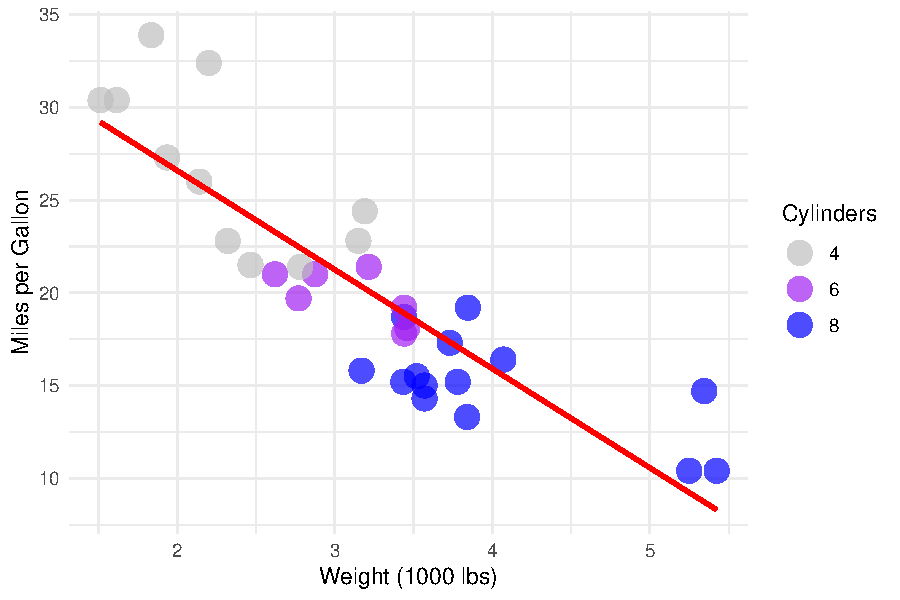
\includegraphics[width=\maxwidth]{figure/scatter-plot-1} \caption[Scatter plot of car weights vs MPG]{Scatter plot of car weights vs MPG}\label{fig:scatter-plot}
\end{figure}

\end{knitrout}

\subsubsection{Analysis}
In Figure~\ref{fig:scatter-plot}, provides insights into the relationship between cars' weight and their MPG, with the added dimension of color-coded cylinders.\\

\textbf{Clusterings}\\
The scatter plot reveals distinct clustering of data points, highlighting specific patterns within the dataset. Cars with four cylinders (color "grey") are predominantly clustered in the lower weight and higher MPG region, representing smaller and more fuel-efficient vehicles. In contrast, cars with eight cylinders (color "blue") tend to be clustered in the higher weight and lower MPG area, indicating larger and less fuel-efficient cars. The identification of this clustering aids in visualising how the number of cylinders influences the trade-off between weight and fuel efficiency.\\

\textbf{Linear Regression Line}\\
The regression line provides a visual representation of the overall relationship between car weight and fuel efficiency.If the line has a positive slope, it indicates that as car weight increases, MPG decreases. Conversely, a negative slope suggests that heavier cars tend to have higher MPG. The steepness of the line represents the strength of this relationship. In this case, the reed regression line indicates a negative correlation—cars tend to have lower fuel efficiency as their weight increases.

\subsubsection{Regression and the Regression Line}
\textbf{Linear regression} is a fundamental statistical method used to model the relationship between a dependent variable (often denoted as \(Y\)) and one or more independent variables (commonly denoted as \(X\)). The objective of linear regression is to find a linear equation that best represents this relationship. In simple linear regression, with one independent variable, the linear regression line is expressed as:

\[
Y = \beta_0 + \beta_1X + \epsilon
\]

Here, \(\beta_0\) is the intercept, \(\beta_1\) is the slope, \(X\) is the independent variable, and \(\epsilon\) represents the error term. The objective of the linear regression line is to minimise the sum of squared differences between the observed and predicted values of \(Y\), which helps us understand how changes in \(X\) affect \(Y\). 

\subsubsection{Bubble Charts}
Bubble charts are a captivating data visualization tool that extends beyond the typical two-dimensional scatter plot by introducing an extra dimension. They represent data points as bubbles or circles on a two-dimensional plane, where the size of each bubble encodes a third variable. This technique enhances data visualization by facilitating the exploration of multivariate data and uncovering patterns that may be hidden in traditional scatter plots.

\textbf{Bubble Chart's Utility in Visualising Data}\\
Bubble charts excel in scenarios where three key variables need to be conveyed simultaneously. The x-axis and y-axis represent two variables, as in a standard scatter plot, while the size of the bubble encodes a third variable, often a quantitative one. This allows for the visualization of relationships between three variables in a single, intuitive graphic.\\
For instance, in economics, bubble charts can illustrate economic indicators, with the x-axis showing time, the y-axis displaying GDP growth, and the bubble size representing a related factor like population or inflation. \\

\textbf{Mathematical Intricacies}\\
The mathematical intricacies of constructing bubble charts involve scaling the data values to determine the size of each bubble accurately. The size of the bubble is typically proportional to the square root of the variable it represents. The choice of scaling method depends on the data distribution and the message the chart aims to convey.

The formula for calculating the bubble size (\(S\)) often involves applying a linear or nonlinear scaling function:

\[
S = k \cdot \sqrt{V}
\]

Where:
\begin{itemize}
\item \(S\) is the size of the bubble,
\item \(V\) is the value of the variable being represented, and
\item \(k\) is a scaling factor to control the bubble size.
\end{itemize}

Selecting an appropriate scaling factor (\(k\)) is critical for maintaining the proportionality between the bubble size and the variable being represented.

\subsubsection{Bubble Charts in Practice}
 This bubble plot visualizes data from the same dataset as above. The purpose of this plot is to depict the relationship between car models and their fuel efficiency (mpg) while using the size of the bubbles to represent the car's horsepower (hp) and color-coding the bubbles based on the number of cylinders (cyl).

\begin{knitrout}
\definecolor{shadecolor}{rgb}{0.969, 0.969, 0.969}\color{fgcolor}\begin{kframe}
\begin{alltt}
\hlcom{#Create bubble plot }
\hlkwd{ggplot}\hlstd{(mtcars,} \hlkwd{aes}\hlstd{(}\hlkwc{x} \hlstd{=} \hlkwd{rownames}\hlstd{(mtcars),} \hlkwc{y} \hlstd{= mpg,} \hlkwc{size} \hlstd{= hp,} \hlkwc{color} \hlstd{= cyl))} \hlopt{+}
  \hlkwd{geom_point}\hlstd{()} \hlopt{+}
  \hlkwd{labs}\hlstd{(}
    \hlkwc{x} \hlstd{=} \hlstr{"Car Models"}\hlstd{,}
    \hlkwc{y} \hlstd{=} \hlstr{"Miles per Gallon"}\hlstd{,}
    \hlkwc{size} \hlstd{=} \hlstr{"Horsepower (hp)"}\hlstd{,}
    \hlkwc{color} \hlstd{=} \hlstr{"Cylinders (cyl)"}
  \hlstd{)} \hlopt{+}
  \hlkwd{scale_size_continuous}\hlstd{(}\hlkwc{range} \hlstd{=} \hlkwd{c}\hlstd{(}\hlnum{3}\hlstd{,} \hlnum{10}\hlstd{))} \hlopt{+}
  \hlkwd{scale_color_gradient}\hlstd{(}\hlkwc{low} \hlstd{=} \hlstr{"lightblue"}\hlstd{,} \hlkwc{high} \hlstd{=} \hlstr{"darkblue"}\hlstd{)} \hlopt{+}
  \hlkwd{theme_minimal}\hlstd{()} \hlopt{+}
  \hlkwd{theme}\hlstd{(}\hlkwc{axis.text.x} \hlstd{=} \hlkwd{element_text}\hlstd{(}\hlkwc{angle} \hlstd{=} \hlnum{90}\hlstd{,} \hlkwc{hjust} \hlstd{=}\hlnum{1}\hlstd{))}
\end{alltt}
\end{kframe}
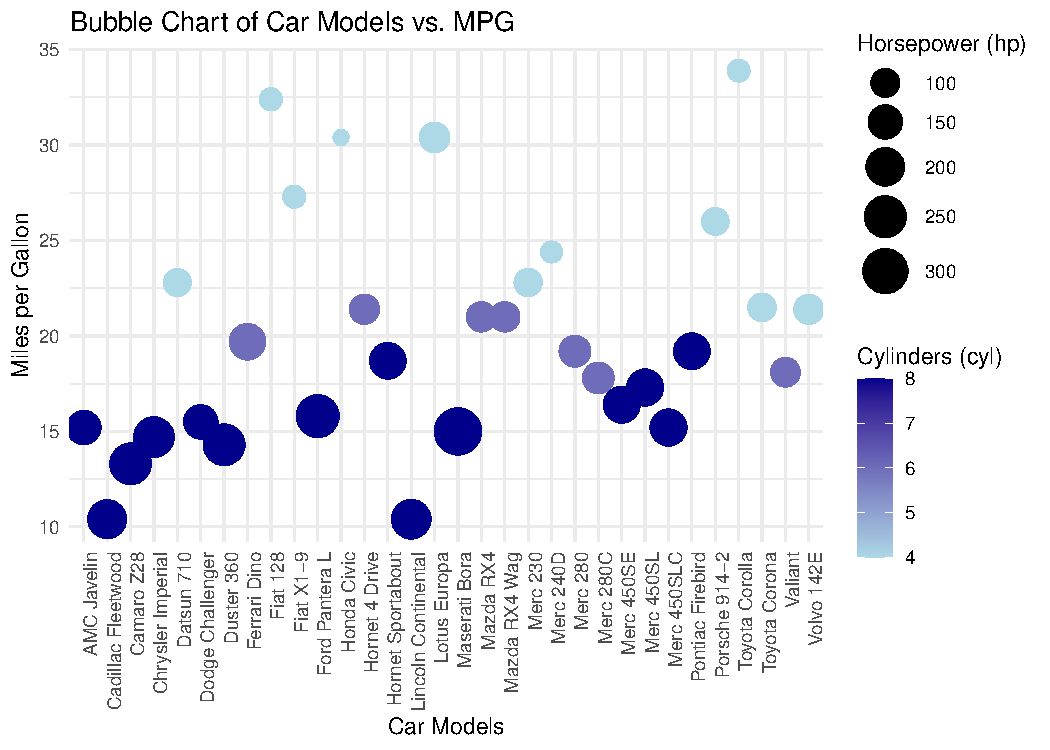
\includegraphics[width=\maxwidth]{figure/buble-plot-chunk-1} 
\end{knitrout}

\subsubsection{Analysis}
The plot's title, axis labels, and legends provide context and clarity to the visualization, making it accessible and informative. Additionally, the choice of a gradient color scale for the number of cylinders enhances the visual appeal and aids in interpreting the data.This bubble plot allows for quick comparisons between multiple characteristics of different car models.The resulting bubble plot effectively conveys several key insights:
\begin{enumerate}
\item \textbf{Car Model vs. MPG}: The x-axis displays the car models, offering a clear representation of each vehicle in the dataset. The bubble plot is particularly useful for displaying nominal data, such as car model names, as it allows easy identification and comparison.
\item \textbf{Miles per Gallon (MPG)}: The y-axis measures miles per gallon, representing the fuel efficiency of each car model. Higher bubbles indicate better fuel efficiency. This variable, which is continuous, is positioned vertically to demonstrate how each car model's fuel efficiency relates to others.
\item \textbf{Horsepower (HP)}: The size of each bubble represents the car's horsepower (hp). Larger bubbles correspond to higher horsepower, providing an additional dimension to the data. The size encoding helps identify more powerful cars.
\item \textbf{Cylinders (Cyl)}: The color of each bubble is determined by the number of cylinders (cyl) in the car's engine. The color scheme adds a categorical aspect to the visualization, making it easy to differentiate between cars with different cylinder counts.
\end{enumerate}


\subsection{Bar Charts and Histograms}
\subsubsection{Bar Charts}
A bar chart is a very important method to present data. It organizes information into vertical bars.  Bar charts have lots of advantages in data visualization. It can present data categories in a frequency distribution. A bar chart is best for comparing classified data. Especially when the values are close, because the human perception of height is better than other visual elements (such as area, angle, etc.), the use of a bar chart is more appropriate. These bars usually have different lengths, and every length is proportional to the size of the information they present.\\
R uses the function $barplot()$ to create bar charts. R can draw both vertical and Horizontal bars in the bar chart. In the bar chart, each of the bars can be given different colors.\\
R is a programming language for data analysis and statistical computing, and its advent has made data visualization more straightforward and accessible. Among the various tools available in R, ggplot2 stands out as one of the most renowned and powerful tools for creating data visualizations. It offers a wealth of data visualization capabilities and is celebrated for its versatility and aesthetic appeal. In this chapter, we will focus on how to use ggplot2 to create bar charts for data visualization.\\

\subsubsection{Different Types of Bar Charts}
Here is an overview of the different types of bar charts. \\
\paragraph{Vertical Bar Chart}
This is the most common bar chart. We use different vertical columns to display and compare the values of different categories in the same dimension, where the X-axis represents the contrasting categories and the Y-axis represents the frequency or count of their categories.\\
\paragraph{Horizontal Bar Chart}
This is very similar to a vertical bar chart but rotated 90 degrees. Categories are shown on the y-axis and frequency or count are shown on the x-axis. Horizontal bar charts are especially useful when category names are long or when there are numerous categories.
\paragraph{Multi-set Bar Chart}
Also known as a grouped bar chart or clustered bar chart. A multi-set bar chart is used to represent and compare different sub-groups within individual categories. This type of chart is useful when you want to show and compare multiple sets of data side-by-side.
Multi-set Bar charts can be horizontal or vertical like the other normal bar charts, and the length of each bar represents the frequency or count of their categories.
\paragraph{Stacked bar chart}
Similar to bar charts, stacked bar charts are often used to compare different classes of values and, within each class of values, are divided into sub-classes, which are often referred to by different colors. Each segment's size is proportional to the frequency or count that it represents from the sub-category. The entire bar's length represents the cumulative total of all the sub-categories.
However, it is very easy to get confused when there are too many categories.

\subsubsection{Advantages of Bar Charts}
\begin{enumerate}
\item \textbf{Clarity and Simplicity}: Bar charts are structurally simple, making them easy to read and understand, allowing audiences to quickly grasp key information.
    \item \textbf{Effective Comparison}: They provide a visual representation that makes comparing the size or value of different categories straightforward, especially when comparing a limited number of categorical data.
    \item \textbf{High Flexibility}: They can be used to represent any type of data, be it continuous or discrete.
    \item \textbf{Multilevel Representation}: Stacked or grouped bar charts can be used to represent multiple data series.
\end{enumerate}

\subsubsection{Disadvantages of Bar Charts}
\begin{enumerate}
    \item \textbf{Limited Data Representation}: They might not be suitable for representing large datasets as things can get cluttered.
    \item \textbf{Potential Misinterpretation}: Without a zero baseline, bar charts can be misleading as they might exaggerate differences.
    \item \textbf{Overcomplexity with Many Categories}: If there are too many bars, it can be challenging to discern information effectively.
    \item \textbf{Requires Categorical Data}: Bar charts are not ideal for representing trends over continuous data, where line graphs might be more appropriate.
\end{enumerate}
\subsubsection{ToothGrowth Dataset}

The \textit{ToothGrowth} dataset is a built-in dataset in R. It is used to study the impact of vitamin C on the tooth growth of Guinea pigs. The dataset consists of 60 observations and 3 variables:

\begin{itemize}
    \item \textbf{len}: Represents the length of the Guinea pigs' teeth.
    \item \textbf{supp}: Indicates the method of vitamin C supplementation, with two levels: "VC" for vitamin C in their diet and "OJ" for vitamin C in orange juice.
    \item \textbf{dose}: Denotes the dosage of vitamin C in milligrams per day, with three levels: 0.5, 1, and 2.
\end{itemize}

This dataset is commonly used for conducting statistical analyses such as analysis of variance (ANOVA) to determine if vitamin C supplementation significantly affects the tooth growth of Guinea pigs. It serves as a typical example for learning statistics and data visualization.

This bar chart illustrates the tooth growth in relation to varying doses of a vitamin. The key observations are:

\begin{enumerate}
    \item \textbf{X-axis Description:} The X-axis represents different dosages of the vitamin (mg/day). There are three distinct dosage levels.
    
    \item \textbf{Y-axis Description:} The Y-axis signifies the length of tooth growth (len). This represents the average tooth growth at the given vitamin dosage.
    \item \textbf{Data Observation:} From the heights of the bars, it is evident that as the vitamin dosage increases, the tooth growth also appears to increase. This might suggest that higher doses of the vitamin may promote tooth growth.
\end{enumerate}
\begin{knitrout}
\definecolor{shadecolor}{rgb}{0.969, 0.969, 0.969}\color{fgcolor}\begin{kframe}
\begin{alltt}
\hlkwd{library}\hlstd{(datasets)}
\hlcom{# load ToothGrowth dataset from R}
\hlkwd{data}\hlstd{(ToothGrowth)}
\hlkwd{ggplot}\hlstd{(ToothGrowth,} \hlkwd{aes}\hlstd{(}\hlkwc{x} \hlstd{=} \hlkwd{factor}\hlstd{(dose),} \hlkwc{y} \hlstd{= len))} \hlopt{+}\hlcom{# Create a bar chart with different vitamin doses on the X-axis and tooth growth on the Y-axis (len).}
  \hlkwd{geom_bar}\hlstd{(}\hlkwc{stat} \hlstd{=} \hlstr{"identity"}\hlstd{,} \hlkwc{position} \hlstd{=} \hlstr{"dodge"}\hlstd{,} \hlkwc{fill} \hlstd{=} \hlstr{"grey"}\hlstd{)} \hlopt{+}
  \hlkwd{labs}\hlstd{(}\hlkwc{title} \hlstd{=} \hlstr{"Tooth Growth by Dose"}\hlstd{,} \hlkwc{x} \hlstd{=} \hlstr{"Dose (mg/day)"}\hlstd{,} \hlkwc{y} \hlstd{=} \hlstr{"Tooth Length"}\hlstd{)} \hlopt{+}
  \hlkwd{theme_minimal}\hlstd{()}
\end{alltt}
\end{kframe}\begin{figure}
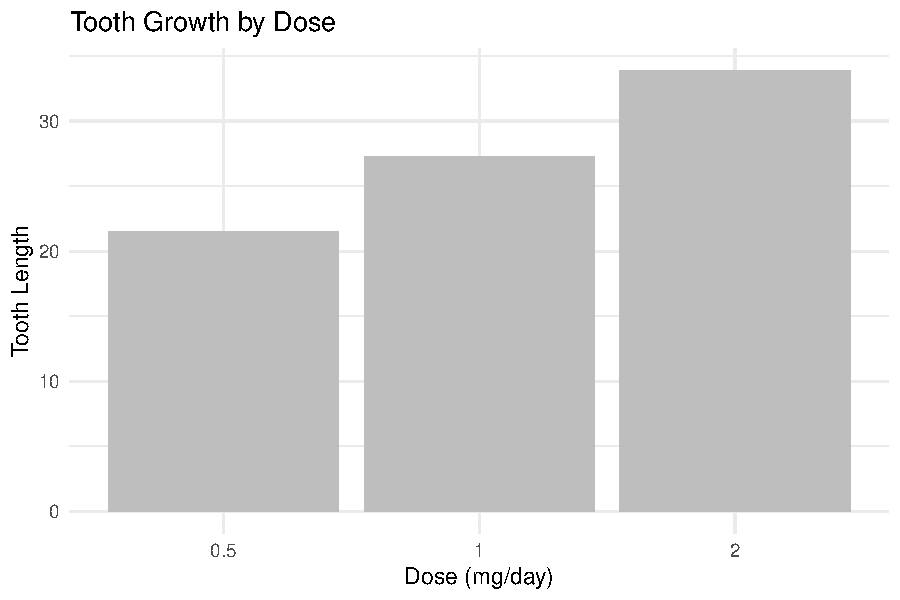
\includegraphics[width=\maxwidth]{figure/barchart1-1} \caption[Tooth growth by dose]{Tooth growth by dose}\label{fig:barchart1}
\end{figure}

\end{knitrout}
The provided bar chart elucidates tooth growth as influenced by varying doses of a vitamin and further differentiates based on the type of supplement. Below are the primary observations:

\begin{enumerate}
    \item \textbf{X-axis Description:} The X-axis categorizes different dosages of the vitamin, with three distinct dosage levels: 0.5, 1, and 2 mg/day.
    
    \item \textbf{Y-axis Description:} The Y-axis measures the length of tooth growth, representing the average growth at the specific vitamin dosage and supplement.
    \item \textbf{Data Observation:} It's discernible from the heights and grouping of the bars that the tooth growth tends to increase with higher doses of the vitamin. However, the effectiveness seems to vary based on the type of supplement. A closer inspection would be required to determine which supplement is more effective at each dosage.
\end{enumerate}

\begin{knitrout}
\definecolor{shadecolor}{rgb}{0.969, 0.969, 0.969}\color{fgcolor}\begin{kframe}
\begin{alltt}
\hlkwd{ggplot}\hlstd{(filtered_data,} \hlkwd{aes}\hlstd{(}\hlkwc{x} \hlstd{=} \hlkwd{factor}\hlstd{(dose),} \hlkwc{y} \hlstd{= len,} \hlkwc{fill} \hlstd{= supp))} \hlopt{+}
  \hlkwd{geom_bar}\hlstd{(}\hlkwc{stat} \hlstd{=} \hlstr{"identity"}\hlstd{,} \hlkwc{position} \hlstd{=} \hlkwd{position_dodge}\hlstd{(}\hlkwc{width} \hlstd{=} \hlnum{0.7}\hlstd{))} \hlopt{+}
  \hlkwd{labs}\hlstd{(}
    \hlkwc{title} \hlstd{=} \hlstr{"Tooth Growth by Dose and Supplement"}\hlstd{,}
    \hlkwc{x} \hlstd{=} \hlstr{"Dose (mg/day)"}\hlstd{,}
    \hlkwc{y} \hlstd{=} \hlstr{"Tooth Length"}\hlstd{,}
    \hlkwc{fill} \hlstd{=} \hlstr{"Supplement"}
  \hlstd{)} \hlopt{+}
  \hlkwd{theme_minimal}\hlstd{()}
\end{alltt}
\end{kframe}\begin{figure}
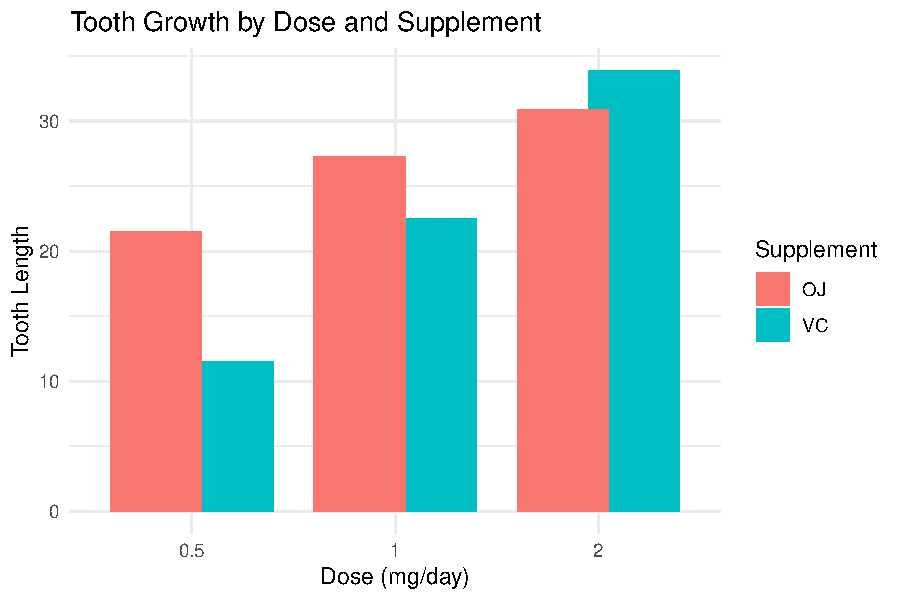
\includegraphics[width=\maxwidth]{figure/barchart2-1} \caption[Tooth Growth by Dose and Supplement(grouping bar chart)]{Tooth Growth by Dose and Supplement(grouping bar chart)}\label{fig:barchart2}
\end{figure}

\end{knitrout}
The displayed bar chart provides insights into tooth growth influenced by varying doses of a vitamin, further categorized by the type of supplement (`supp`). The key insights from this chart are:

\begin{enumerate}
    \item \textbf{X-axis Description:} The X-axis demarcates different vitamin dosages, categorized into three distinct levels: 0.5, 1, and 2 mg/day.
    
    \item \textbf{Y-axis Description:} The Y-axis quantifies tooth growth length, representing the combined average growth for both supplements at the respective vitamin dosages.
    \item \textbf{Data Observation:} The total height of each bar signifies the combined tooth growth for both supplements at the given dosage. From the stacked sections, it's evident that the impact on tooth growth varies based on the supplement type. A detailed inspection might elucidate the relative effectiveness of the supplements at each dosage level.
\end{enumerate}
\begin{knitrout}
\definecolor{shadecolor}{rgb}{0.969, 0.969, 0.969}\color{fgcolor}\begin{kframe}
\begin{alltt}
\hlkwd{ggplot}\hlstd{(filtered_data,} \hlkwd{aes}\hlstd{(}\hlkwc{x} \hlstd{=} \hlkwd{factor}\hlstd{(dose),} \hlkwc{y} \hlstd{= len,} \hlkwc{fill} \hlstd{= supp))} \hlopt{+}
  \hlkwd{geom_bar}\hlstd{(}\hlkwc{stat} \hlstd{=} \hlstr{"identity"}\hlstd{,} \hlkwc{position} \hlstd{=} \hlstr{"stack"}\hlstd{)} \hlopt{+}
  \hlkwd{labs}\hlstd{(}
    \hlkwc{title} \hlstd{=} \hlstr{"Tooth Growth by Dose and Supplement"}\hlstd{,}
    \hlkwc{x} \hlstd{=} \hlstr{"Dose (mg/day)"}\hlstd{,}
    \hlkwc{y} \hlstd{=} \hlstr{"Tooth Length"}\hlstd{,}
    \hlkwc{fill} \hlstd{=} \hlstr{"Supplement"}
  \hlstd{)} \hlopt{+}
  \hlkwd{theme_minimal}\hlstd{()}
\end{alltt}
\end{kframe}\begin{figure}
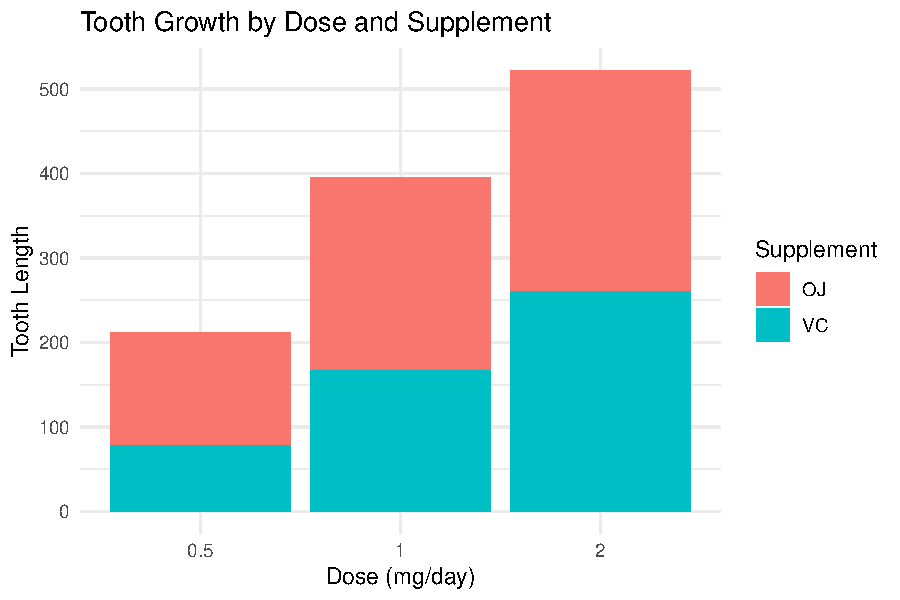
\includegraphics[width=\maxwidth]{figure/bar_chat3-1} \caption[Tooth Growth by Dose and Supplement(stacked bar chart)]{Tooth Growth by Dose and Supplement(stacked bar chart)}\label{fig:bar chat3}
\end{figure}

\end{knitrout}
In the next part of our section, we will look at another plot which called Histogram.
\subsubsection{Histograms}
Histograms, although visually similar to bar charts, convey different meanings. A histogram involves concepts of statistics. It requires data to be categorized into groups and then counts the data points within each of those groups. On a Cartesian coordinate system, the x-axis shows the endpoints of each group, and the y-axis represents frequency. The height of each rectangle indicates the corresponding frequency, making it a frequency distribution histogram. In order to determine the quantity of each group in the histogram, a multiplication of the frequency by the group interval is necessary. Since every histogram has a fixed group interval, if we use the y-axis to directly show quantity and each rectangle's height indicates the number of data points, we can both retain the distribution and simultaneously see the number in each group at a glance. All examples in this text use the non-standard histogram depiction with the y-axis denoting quantity.

\subsubsection{Uses of Histograms:}
Histograms demonstrates the distribution of frequency or quantity across groups.\\
Facilitates the visualization of differences in frequency or quantity among groups.\\
The R language uses the $hist()$ function to create histograms. This function takes vectors as input and uses a few more parameters to plot the histogram.\\
Now, we want to creat a better graph with ggplot2 thanks to the $geom_histogram()$ function and iris dataset.\\
The iris dataset is a classic dataset in the field of statistics. It was introduced by the British biologist Ronald A. Fisher in 1936 as an example of discriminant analysis. The dataset consists of 150 samples from three species of iris flowers: setosa, versicolor, and virginica. For each sample, four features were measured: the lengths and the widths of the sepals and petals, all in centimeters. The dataset is often used for classification tasks to differentiate between the three species based on the given measurements. It has become a standard test case for many classification algorithms and is widely recognized in the data science community.\\
\begin{knitrout}
\definecolor{shadecolor}{rgb}{0.969, 0.969, 0.969}\color{fgcolor}\begin{kframe}
\begin{alltt}
\hlstd{bar_diagram} \hlkwb{<-} \hlkwd{ggplot}\hlstd{(iris,} \hlkwd{aes}\hlstd{(}\hlkwc{x} \hlstd{= Sepal.Length))} \hlopt{+}
  \hlkwd{geom_histogram}\hlstd{(}
    \hlkwc{binwidth} \hlstd{=} \hlnum{0.2}\hlstd{,}  \hlcom{# Adjust the box width to 0.2 for smaller data sets}
    \hlkwc{fill} \hlstd{=} \hlstr{"grey"}\hlstd{,}
    \hlkwc{color} \hlstd{=} \hlstr{"black"}
  \hlstd{)} \hlopt{+}
  \hlkwd{labs}\hlstd{(}
    \hlkwc{title} \hlstd{=} \hlstr{"Histogram of Sepal Length in Iris Dataset"}\hlstd{,}
    \hlkwc{x} \hlstd{=} \hlstr{"Sepal Length/cm"}\hlstd{,}
    \hlkwc{y} \hlstd{=} \hlstr{"Frequency"}
  \hlstd{)} \hlopt{+}
  \hlkwd{theme_minimal}\hlstd{()}
\hlkwd{print}\hlstd{(bar_diagram)}
\end{alltt}
\end{kframe}\begin{figure}
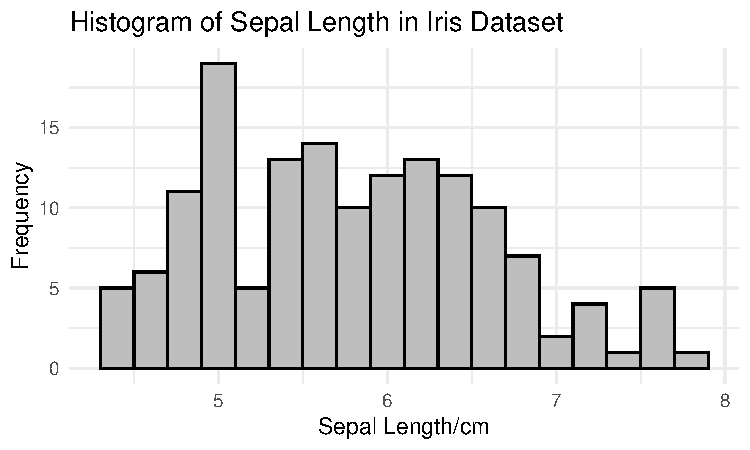
\includegraphics[width=\maxwidth]{figure/hist3-1} \caption[Histogram of Sepal Length in Iris Dataset]{Histogram of Sepal Length in Iris Dataset}\label{fig:hist3}
\end{figure}

\end{knitrout}

\subsection{Heatmaps and Tree Maps}
In this chapter, we explore two powerful data visualisation techniques: heatmaps and treemaps. These methods are instrumental for conveying intricate data structures and patterns, offering unique ways to represent multivariate information, making them indispensable tools for data scientists.
\\  
\\We will delve into the theory behind heatmaps and treemaps, understand how to create them using popular data visualization libraries, and demonstrate their practical applications with real-world examples. By the end of this chapter, you will be well-equipped to leverage heatmaps and treemaps to gain insights from complex and hierarchical datasets.
\subsubsection{Heatmaps - Fire in Brazil}
\\  
\\The heatmap is a data visualisation technique that uses colour coding to represent different intensity.
\\  
<<<<<<< HEAD
\\In this illustrative example, heatmaps are used to visualise fire occurrences in Brazil. These heatmaps provide a spatially coherent representation, highlighting regions at high risk and seasonal patterns. Here, the heatmap is a powerful tool for identifying the occurrence of fire incidents. The data-driven insights could empower policymakers to make informed decisions regarding preventive measures and firefighting strategies.
=======
\\In this illustrative example, heatmaps is used to visualize fire occurrences in Brazil. These heatmaps offer a spatially coherent representation, highlighting regions at high risk and seasonal patterns. Here, the heatmap is a power tool for identifying the risk of fire incidents. The data-driven insights empowers us to make informed decisions concerning preventive measures and strategies for firefighting.





\\From Figure~\ref{fig:spacetime-fy22}, we can observe that certain locations have significantly higher fires count. 
>>>>>>> daff6d291b446528a6d1466dc3e93744c22fdbf7
\\  
\\In Figure~\ref{fig:spacetime-fy22}, it can be observed that significantly higher fire counts are found in certain locations. The presence of two strips with high frequencies of fires are highly unusual.  The vertical trend corresponds to the location of BR-230 (Trans-Amazonian Highway) passing through the city of Apuí, State of Amazonas, where a high frequency of fire occurrence is observed.  The horizontal trend corresponds to BR-163 (Brazil highway) passing through Três Pinheiros in Novo Progresso, State of Pará. The western coastal area with a high frequency of fire occurrence corresponds to regions in close proximity to the cities of Vista Alegre do Abunã and Rio Branco. Research has indicated that 95 \% of active fires and the most intense ones (FRP > 500 megawatts) occurred at the edges in forests.
\\  
\\From the same figure, it can be observed that August and September are the riskiest months in terms of fire hazard, whereas little risk is posed from November to July. The follow-up question naturally arises: How does FY22 compare to previous years? Is it valid to claim that August and September constitute the fire hazard season?
\\    
\\In Figure~\ref{fig:fire-by-months-fy13-22}, the data shows a higher number of fire occurrences in the months of August to October compared to the rest of the year, indicating a greater number of fire hazards during these months.
\\  






\begin{knitrout}
\definecolor{shadecolor}{rgb}{0.969, 0.969, 0.969}\color{fgcolor}\begin{kframe}
\begin{alltt}
\hlcom{# Obtain the Brazil map data}
\hlstd{brazil_map} \hlkwb{<-} \hlkwd{map_data}\hlstd{(}\hlstr{"world"}\hlstd{,} \hlkwc{region} \hlstd{=} \hlstr{"Brazil"}\hlstd{)}

\hlcom{# Create the heatmap of fire occurrences}
\hlstd{space_heatmap} \hlkwb{<-} \hlkwd{ggplot}\hlstd{(confident_fire_fy22,} \hlkwd{aes}\hlstd{(}\hlkwc{x} \hlstd{= longitude,} \hlkwc{y} \hlstd{= latitude))} \hlopt{+}
  \hlkwd{geom_polygon}\hlstd{(}\hlkwc{data} \hlstd{= brazil_map,} \hlkwd{aes}\hlstd{(}\hlkwc{x} \hlstd{= long,} \hlkwc{y} \hlstd{= lat,} \hlkwc{group} \hlstd{= group),}
               \hlkwc{fill} \hlstd{=} \hlstr{"#bdbdbd"}\hlstd{)} \hlopt{+}
  \hlkwd{geom_bin2d}\hlstd{(}\hlkwc{bins} \hlstd{=} \hlnum{300}\hlstd{)} \hlopt{+}
  \hlkwd{scale_fill_gradient}\hlstd{(}\hlkwc{low} \hlstd{=} \hlstr{"#fee6ce"}\hlstd{,} \hlkwc{high} \hlstd{=} \hlstr{"#d7301f"}\hlstd{)} \hlopt{+}
  \hlkwd{coord_fixed}\hlstd{(}\hlkwc{ratio} \hlstd{=} \hlnum{1}\hlstd{)} \hlopt{+}
  \hlkwd{theme_minimal}\hlstd{()}\hlopt{+}
  \hlkwd{theme}\hlstd{(}\hlkwc{axis.text} \hlstd{=} \hlkwd{element_text}\hlstd{(}\hlkwc{size} \hlstd{=} \hlnum{9}\hlstd{))}

\hlstd{interactive_plot} \hlkwb{<-} \hlkwd{ggplotly}\hlstd{(space_heatmap)}

\hlstd{time_heatmap} \hlkwb{<-} \hlkwd{ggplot}\hlstd{(confident_fire_months_fy22,}
                       \hlkwd{aes}\hlstd{(}\hlkwc{x} \hlstd{= abb_month,} \hlkwc{y} \hlstd{=} \hlkwd{as.character}\hlstd{(}\hlnum{2022}\hlstd{),} \hlkwc{fill} \hlstd{= count))} \hlopt{+}
  \hlkwd{geom_tile}\hlstd{(}\hlkwc{width} \hlstd{=} \hlnum{0.9}\hlstd{,} \hlkwc{height} \hlstd{=} \hlnum{0.5}\hlstd{)} \hlopt{+}  \hlcom{# Create the heatmap tiles}
  \hlkwd{scale_fill_gradient}\hlstd{(}\hlkwc{low} \hlstd{=} \hlstr{"#fff7ec"}\hlstd{,} \hlkwc{high} \hlstd{=} \hlstr{"#d7301f"}\hlstd{)} \hlopt{+}
  \hlkwd{labs}\hlstd{(}\hlkwc{x} \hlstd{=} \hlstr{" "}\hlstd{,} \hlkwc{y} \hlstd{=} \hlstr{" "}\hlstd{,} \hlkwc{name} \hlstd{=} \hlstr{"count"}\hlstd{)} \hlopt{+}
  \hlkwd{theme_minimal}\hlstd{()} \hlopt{+}
  \hlkwd{theme}\hlstd{(}\hlkwc{axis.text} \hlstd{=} \hlkwd{element_text}\hlstd{(}\hlkwc{size} \hlstd{=} \hlnum{9}\hlstd{))}

\hlstd{spacetime_fy22} \hlkwb{<-} \hlkwd{grid.arrange}\hlstd{(space_heatmap, time_heatmap,} \hlkwc{nrow} \hlstd{=} \hlnum{2}\hlstd{,}
                               \hlkwc{heights} \hlstd{=} \hlkwd{c}\hlstd{(}\hlnum{2}\hlstd{,}\hlnum{0.5}\hlstd{))}

\hlkwd{print}\hlstd{(spacetime_fy22)}
\end{alltt}
\begin{verbatim}
## TableGrob (2 x 1) "arrange": 2 grobs
##   z     cells    name           grob
## 1 1 (1-1,1-1) arrange gtable[layout]
## 2 2 (2-2,1-1) arrange gtable[layout]
\end{verbatim}
\end{kframe}\begin{figure}
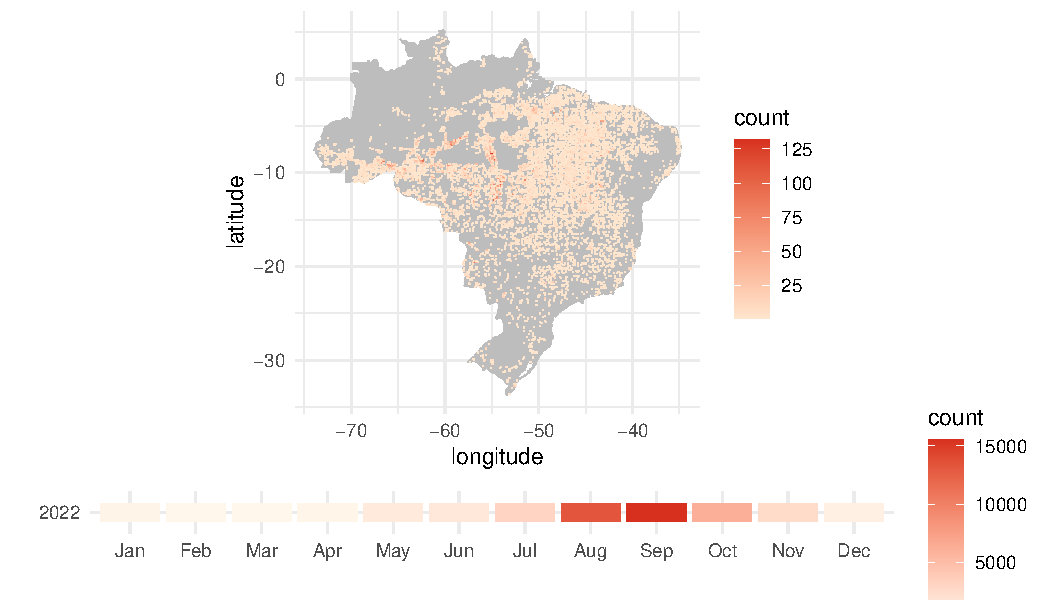
\includegraphics[width=\maxwidth]{figure/spacetime-fy22-1} \caption[Frequency of Fire by Space and Time, FY22]{Frequency of Fire by Space and Time, FY22}\label{fig:spacetime-fy22}
\end{figure}

\end{knitrout}




\begin{knitrout}
\definecolor{shadecolor}{rgb}{0.969, 0.969, 0.969}\color{fgcolor}\begin{kframe}
\begin{alltt}
\hlstd{heatmap_plot} \hlkwb{<-} \hlkwd{ggplot}\hlstd{(pivot_table,}
                       \hlkwd{aes}\hlstd{(}\hlkwc{x} \hlstd{=} \hlkwd{factor}\hlstd{(abb_month,} \hlkwc{levels} \hlstd{= custom_order),}
                           \hlkwc{y} \hlstd{=} \hlkwd{as.character}\hlstd{(year),} \hlkwc{fill} \hlstd{= count))} \hlopt{+}
  \hlkwd{geom_tile}\hlstd{()} \hlopt{+}
  \hlkwd{scale_fill_gradient}\hlstd{(}\hlkwc{low} \hlstd{=} \hlstr{"#fff7ec"}\hlstd{,} \hlkwc{high} \hlstd{=} \hlstr{"#d7301f"}\hlstd{)} \hlopt{+}
  \hlkwd{labs}\hlstd{(}\hlkwc{x} \hlstd{=} \hlstr{" "}\hlstd{,} \hlkwc{y} \hlstd{=} \hlstr{" "}\hlstd{)} \hlopt{+}
  \hlkwd{theme_minimal}\hlstd{()} \hlopt{+}
  \hlkwd{theme}\hlstd{(}\hlkwc{axis.text} \hlstd{=} \hlkwd{element_text}\hlstd{(}\hlkwc{size} \hlstd{=} \hlnum{9}\hlstd{))}

\hlkwd{print}\hlstd{(heatmap_plot)}
\end{alltt}
\end{kframe}\begin{figure}
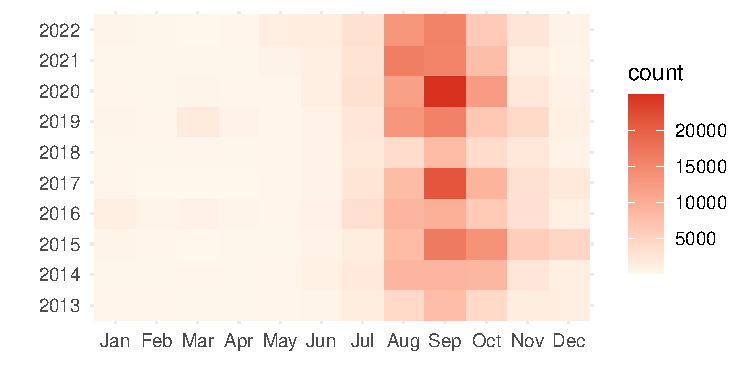
\includegraphics[width=\maxwidth]{figure/fire-by-months-fy13-22-1} \caption[Frequency of Fire Occurrences, FY13-22]{Frequency of Fire Occurrences, FY13-22}\label{fig:fire-by-months-fy13-22}
\end{figure}

\end{knitrout}


\subsubsection{Heatmaps, correlation matrix and AIC score}
\\  
\\The foundation of a heatmap is a data matrix $M$, where each entry in this matrix represents an observation.
$$M =
\left[
\begin{array}{cccc}
    M_{11} & M_{12} & \ldots & M_{1j} \\  
    M_{21} & M_{22} & \ldots & M_{2j} \\  
    \vdots & \vdots & \ddots & \vdots \\  
    M_{i1} & M_{i2} & \ldots & M_{ij}
\end{array}
\right]
$$
\\Therefore, the first step to create a heatmap is to organize the data into columns and rows. In Figure~\ref{fig:fire-by-months-fy13-22}, the structured data is displayed as a grid of coloured cells, where the colour intensity corresponds to the underlying frequency.
\\  
\\Heatmaps serve as powerful tools for visualizing relationships between covariables within a model. An example of the necessity to analyze a matrix of correlations between variables is found in regression models. In the real world, variables are often correlated, and completely independent relationships are seldom encountered. Therefore, the analysis of pairwise correlations becomes essential. Significantly impacted by highly correlated variables, the regression model requires the selection of one variable from the correlated set. The selection is based on the identification of a regression model with the lowest Akaike Information Criterion (AIC) score among these variables. 

$$AIC = -2 \l(\hat{\mathbf{\theta}})+2 \dim (\mathbf{\theta})$$
\\where $\l(\hat{\mathbf{\theta}})$ is the log-likelihood function, which is used to find the Maximum Likelihood Estimator (MLE) of a distribution.
\\  
\\The AIC measures the extent to which the linear model fits the dataset. To obtain the best model, minimise the AIC score. In other words, the objective is to have the trend explained by the regression model, while avoiding overfitting that captures the noise in the dataset, ultimately leading to inaccurate predictions, as demonstrated in Figure \ref{fig:noisy}.

\begin{figure}[h]
    \centering
    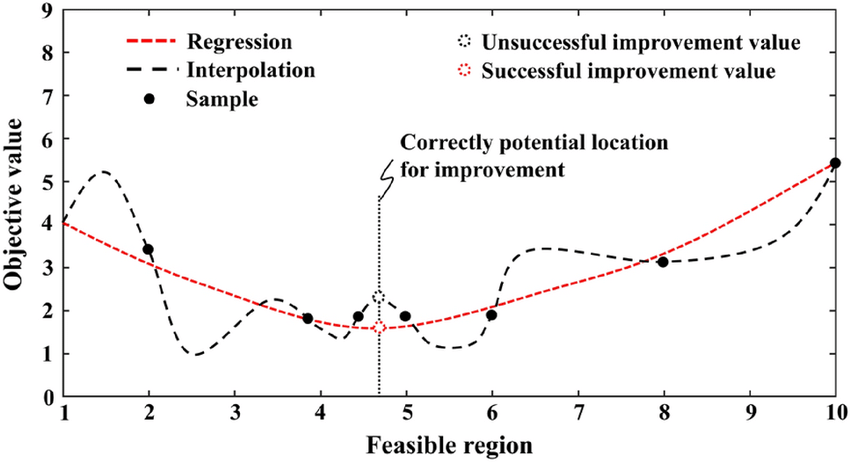
\includegraphics[width=0.7\textwidth]{https://github.com/Qinqing-Li/Data-Visualisation-Project/blob/main/overfitting.png?raw=true}
    \caption{Danger of overfitting the regression model}
    \label{fig:noisy}
\end{figure}

\subsubsection{Treemaps}
Treemaps are a visualisation method specifically designed for hierarchical data structures. They represent data as nested rectangles, where each rectangle represents a part of the whole. Treemaps offer a visually appealing and efficient way to convey the hierarchical composition of data. The size and color of each rectangle can be used to encode additional information.

\subsubsection{Use Cases for Treemaps}
Treemaps are highly effective when dealing with hierarchical data. Some common use cases include:
\begin{itemize}
\item \textbf{Disk Space Visualization}: Treemaps can be employed to visualize disk space usage, where the outermost rectangle represents the entire disk, and inner rectangles represent folders and files. The size of each rectangle reflects the space they occupy.
\item \textbf{Market Share Analysis}: In business, treemaps are useful for visualizing market share data. The top-level rectangle represents the total market, and inner rectangles represent individual segments, brands, or products. The size and color of each segment can represent its share and performance.
\end{itemize}

XXX %missing Treemaps


\subsection{Line Charts and Time Series Visualization}

In this chapter, we are going to investigate the intricacies of the line chart and its most common application: time series. A line chart is a statistical representation that employs a Cartesian coordinate system to depict changes in numerical values over continuous time intervals or ordered categories. The x-axis typically represents these intervals or categories, while the y-axis conveys quantified data. Any negative data values are plotted below the y-axis, and lines are used to connect adjacent data points.
Line graphs are used to analyze trends in things that change over time or ordered categories. If there are multiple sets of data, they are used to analyze the interaction and impact of these data sets over time or ordered categories. The direction of the line represents positive/negative changes, and the slope of the line indicates the degree of change. In terms of data, a line graph requires a continuous time field or a categorical field and at least one continuous data field.\\\\
\textbf{Suitability for Displaying Trends Over Time:}\\
Line charts effectively visualize data trends over time. By plotting data at intervals like days or years, they highlight trends and patterns. Multiple lines on one chart enable easy data comparison, such as contrasting sales of two products. They aid in recognizing seasonal changes, cyclic events, and unexpected shifts, making them invaluable for forecasting. Due to their simplicity, they're accessible to those with minimal data analysis background. Line charts are a prime choice for time series visualization.

Time series visualization is essential in data analysis, showcasing time-ordered data. It reveals long-term trends, helping analysts discern patterns for future planning. It's crucial for spotting seasonality in datasets, especially in sectors like retail. This method also identifies anomalies, suggesting areas needing investigation. Predictive modeling, based on historical patterns, becomes feasible, fostering proactive choices. Overlaying multiple data series offers richer comparative analysis. Overall, time series visualization provides quick insights into chronological data, driving informed decisions by highlighting trends, seasonal changes, and outliers.\\\\
\textbf{Limitations:}\\
While line charts are excellent for displaying trends over time, they have limitations. They may not be suitable for showing individual data distributions or for data where there's no logical order. eg. too many points, too many lines, too many zeros.

\subsubsection{Showcase real-world examples of time series visualisations}

Time series of the daily CNY, CAN, EUR, HKD, USD versus GBP exchange reference rate data
published by the European Central Bank over the time period from 01 Jan 2013 to 12 Oct 2023 (without weekends). The exchange rate tells you how many pounds you need to buy/sell 1 CNY, CAN, EUR, HKD, USD.\\

\textbf{The data set has the format as below:}\\

\begin{table}[h]
\centering
\begin{tabular}{|c|c|c|c|c|c|}
\hline
\textbf{Date} & \textbf{CNYtoGBP} & \textbf{CANtoGBP} & \textbf{EURtoGBP} & \textbf{HKDtoGBP} & \textbf{USDtoGBP} \\
\hline
\%d-\%m-\%y & Value & Value & Value & Value & Value \\
\hline
\end{tabular}
\caption{Field Information: CNY, CAN, EUR, HKD, USD to GBP}
\end{table}

First, we are going to plot all exchange rates in one figure.




\begin{knitrout}
\definecolor{shadecolor}{rgb}{0.969, 0.969, 0.969}\color{fgcolor}\begin{kframe}
\begin{alltt}
\hlcom{# Plot exchange rates of CNY, CAN, EUR, HKD, USD to GBP}
\hlstd{plot_dt} \hlkwb{<-} \hlstd{MyData} \hlopt \hlkwd{gather}\hlstd{(}\hlkwc{key}\hlstd{=}\hlstr{"Currency"}\hlstd{,} \hlkwc{value}\hlstd{=}\hlstr{"Rate"}\hlstd{,} \hlopt{-}\hlstd{Date)}

\hlkwd{ggplot}\hlstd{(plot_dt,} \hlkwd{aes}\hlstd{(}\hlkwc{x}\hlstd{=Date,} \hlkwc{y}\hlstd{=Rate,} \hlkwc{color}\hlstd{=Currency))} \hlopt{+}
  \hlkwd{geom_line}\hlstd{()} \hlopt{+}
  \hlkwd{labs}\hlstd{(}\hlkwc{title}\hlstd{=}\hlstr{"Exchange rates of CNY, CAN, EUR, HKD, USD to GBP"}\hlstd{,}
       \hlkwc{y}\hlstd{=}\hlstr{"Exchange Rate to GBP"}\hlstd{,}
       \hlkwc{x}\hlstd{=}\hlstr{"Date"}\hlstd{,}
       \hlkwc{color}\hlstd{=}\hlstr{"Currency"}\hlstd{)}
\end{alltt}
\end{kframe}\begin{figure}
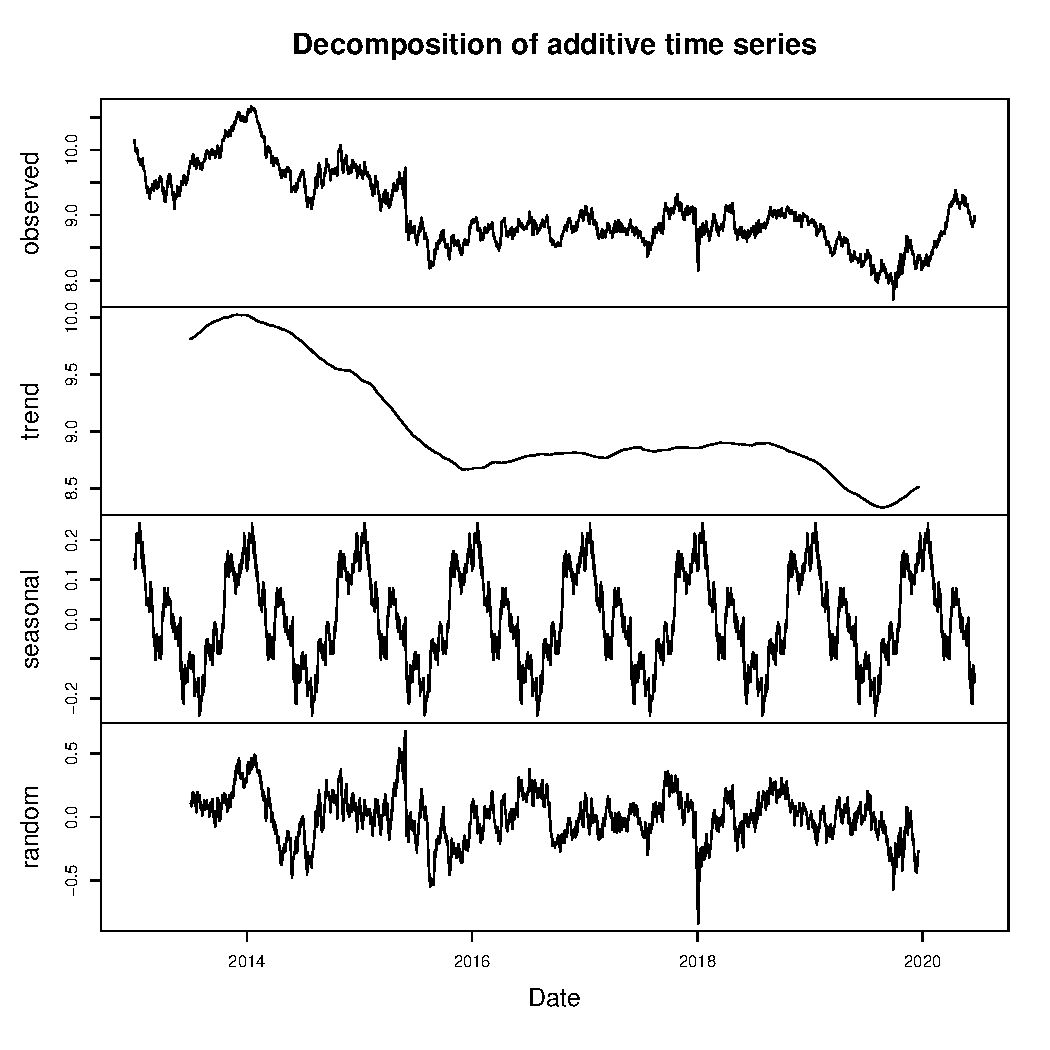
\includegraphics[width=\maxwidth]{figure/unnamed-chunk-2-1} \caption[Exchange rates of CNY, CAN, EUR, HKD, USD to GBP]{Exchange rates of CNY, CAN, EUR, HKD, USD to GBP}\label{fig:unnamed-chunk-2}
\end{figure}

\end{knitrout}


From above plot, we can see the the daily CNY, CAN, EUR, HKD, USD versus GBP exchange in the same plot, which provide us an overview of the trend and comparison. Then we can make the plot smooth by taking averages, which enables easier recognition of trend.


\begin{knitrout}
\definecolor{shadecolor}{rgb}{0.969, 0.969, 0.969}\color{fgcolor}\begin{kframe}
\begin{alltt}
\hlcom{# Calculate 21-day moving average for each currency}
\hlstd{columns} \hlkwb{<-} \hlkwd{names}\hlstd{(MyData)[}\hlopt{!}\hlkwd{names}\hlstd{(MyData)} \hlopt \hlstr{"Date"}\hlstd{]}
\hlkwa{for} \hlstd{(col} \hlkwa{in} \hlstd{columns) \{}
  \hlstd{new_col_name} \hlkwb{<-} \hlkwd{paste0}\hlstd{(col,} \hlstr{"_MA21"}\hlstd{)}
  \hlstd{MyData[[new_col_name]]} \hlkwb{<-} \hlstd{zoo}\hlopt{::}\hlkwd{rollapply}\hlstd{(MyData[[col]],}
                                           \hlkwc{width}\hlstd{=}\hlnum{21}\hlstd{,} \hlkwc{FUN}\hlstd{=mean,}
                                           \hlkwc{fill}\hlstd{=}\hlnum{NA}\hlstd{,} \hlkwc{align}\hlstd{=}\hlstr{'right'}\hlstd{)}
\hlstd{\}}

\hlcom{# Plot 21-day moving average for each currency}
\hlstd{plot_data} \hlkwb{<-} \hlstd{MyData} \hlopt \hlkwd{gather}\hlstd{(}\hlkwc{key}\hlstd{=}\hlstr{"Currency"}\hlstd{,} \hlkwc{value}\hlstd{=}\hlstr{"Rate"}\hlstd{,} \hlopt{-}\hlstd{Date)} \hlopt
  \hlkwd{filter}\hlstd{(}\hlkwd{grepl}\hlstd{(}\hlstr{"MA21"}\hlstd{, Currency))}

\hlkwd{ggplot}\hlstd{(plot_data,} \hlkwd{aes}\hlstd{(}\hlkwc{x}\hlstd{=Date,} \hlkwc{y}\hlstd{=Rate,} \hlkwc{color}\hlstd{=Currency))} \hlopt{+}
  \hlkwd{geom_line}\hlstd{()} \hlopt{+}
  \hlkwd{labs}\hlstd{(}\hlkwc{title}\hlstd{=}\hlstr{"21-Day moving average of exchange rates"}\hlstd{,}
       \hlkwc{y}\hlstd{=}\hlstr{"Exchange Rate to GBP"}\hlstd{,}
       \hlkwc{x}\hlstd{=}\hlstr{"Date"}\hlstd{,}
       \hlkwc{color}\hlstd{=}\hlstr{"Currency"}\hlstd{)}
\end{alltt}
\end{kframe}\begin{figure}
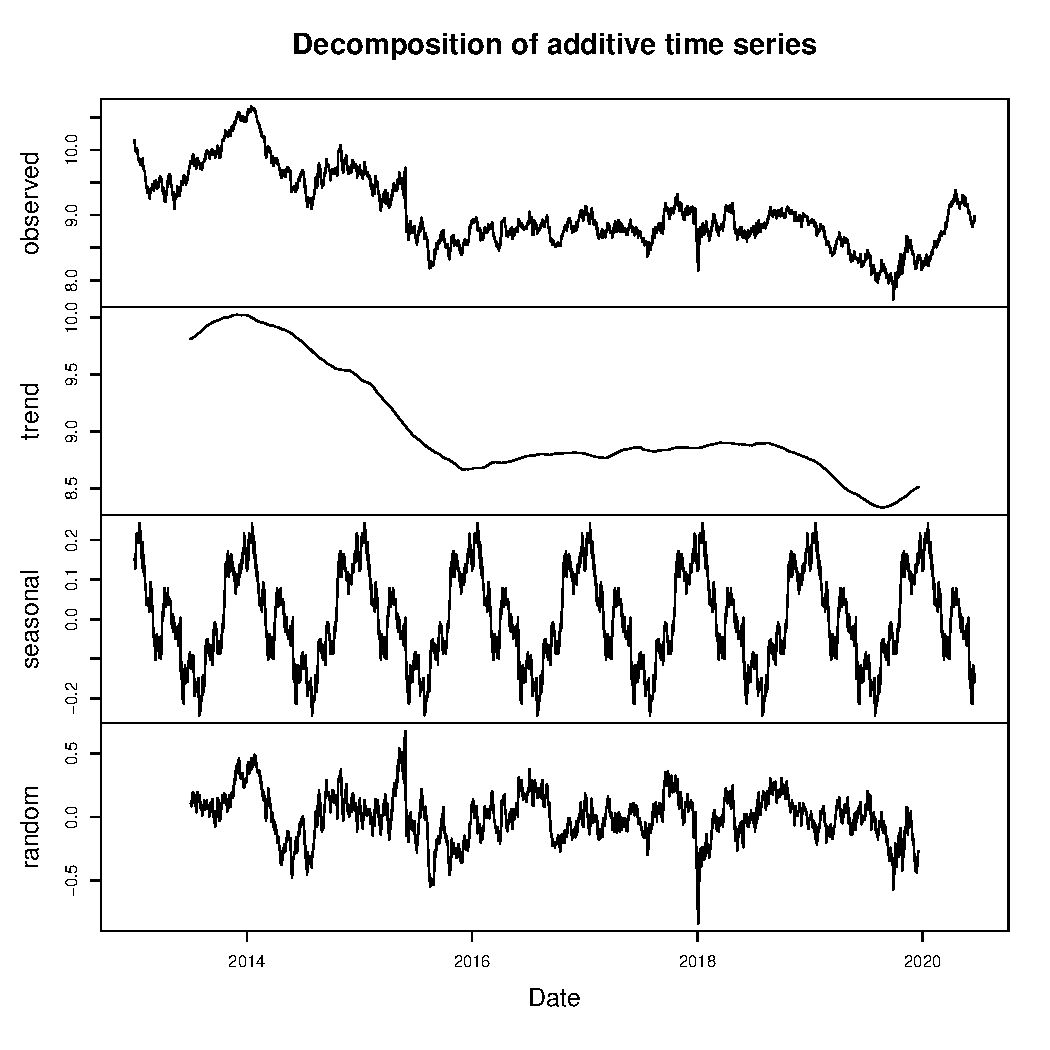
\includegraphics[width=\maxwidth]{figure/unnamed-chunk-3-1} \caption[21-day moving average of exchange rates of CNY, CAN, EUR, HKD, USD to GBP]{21-day moving average of exchange rates of CNY, CAN, EUR, HKD, USD to GBP}\label{fig:unnamed-chunk-3}
\end{figure}

\end{knitrout}

From above plot, a 21-day moving average for each currency allows us to view the trend easily.

\subsubsection{Decomposition of one time series into trend, seasonal, and random.}

One of the primary advantages of time series visualization is the ease with which it allows analysts to identify long-term upward or downward trends in data and patterns that repeat over specific intervals. By decomposing the time series, it would be easy to see those features.

Time series data, $Y_t$, can often be described as a combination of several distinct components:
\begin{itemize}
    \item \textbf{Trend ($T_t$):} The underlying progression in the series.
    \item \textbf{Seasonal ($S_t$):} Periodic fluctuations due to seasonal factor.
    \item \textbf{Residual ($R_t$):} The irregular or error component.
\end{itemize}

The decomposition of a time series can be described in two main models:

Additive Model:
In the additive model, the components are added together:
\[
Y_t = T_t + S_t + R_t
\]

Multiplicative Model:
In the multiplicative model, the components are multiplied together:
\[
Y_t = T_t \times S_t \times R_t
\]

In practice, the choice between the additive and multiplicative models often depends on the nature of the time series. If the magnitude of the seasonal fluctuations or the variation around the trend does not vary with the level of the time series, then an additive model is appropriate. If the magnitude of the seasonal fluctuations or the variation around the trend increases or decreases as the time series level changes, then a multiplicative model may be more suitable.

\begin{knitrout}
\definecolor{shadecolor}{rgb}{0.969, 0.969, 0.969}\color{fgcolor}\begin{kframe}
\begin{alltt}
\hlcom{# Plot decomposition of addictive time series model}
\hlstd{decomposed_ts} \hlkwb{<-} \hlstd{stats}\hlopt{::}\hlkwd{decompose}\hlstd{(ts_data}\hlopt{$}\hlstd{CNYtoGBP)}
\hlkwd{plot}\hlstd{(decomposed_ts,} \hlkwc{xlab}\hlstd{=}\hlstr{"Date"}\hlstd{)}
\end{alltt}
\end{kframe}\begin{figure}
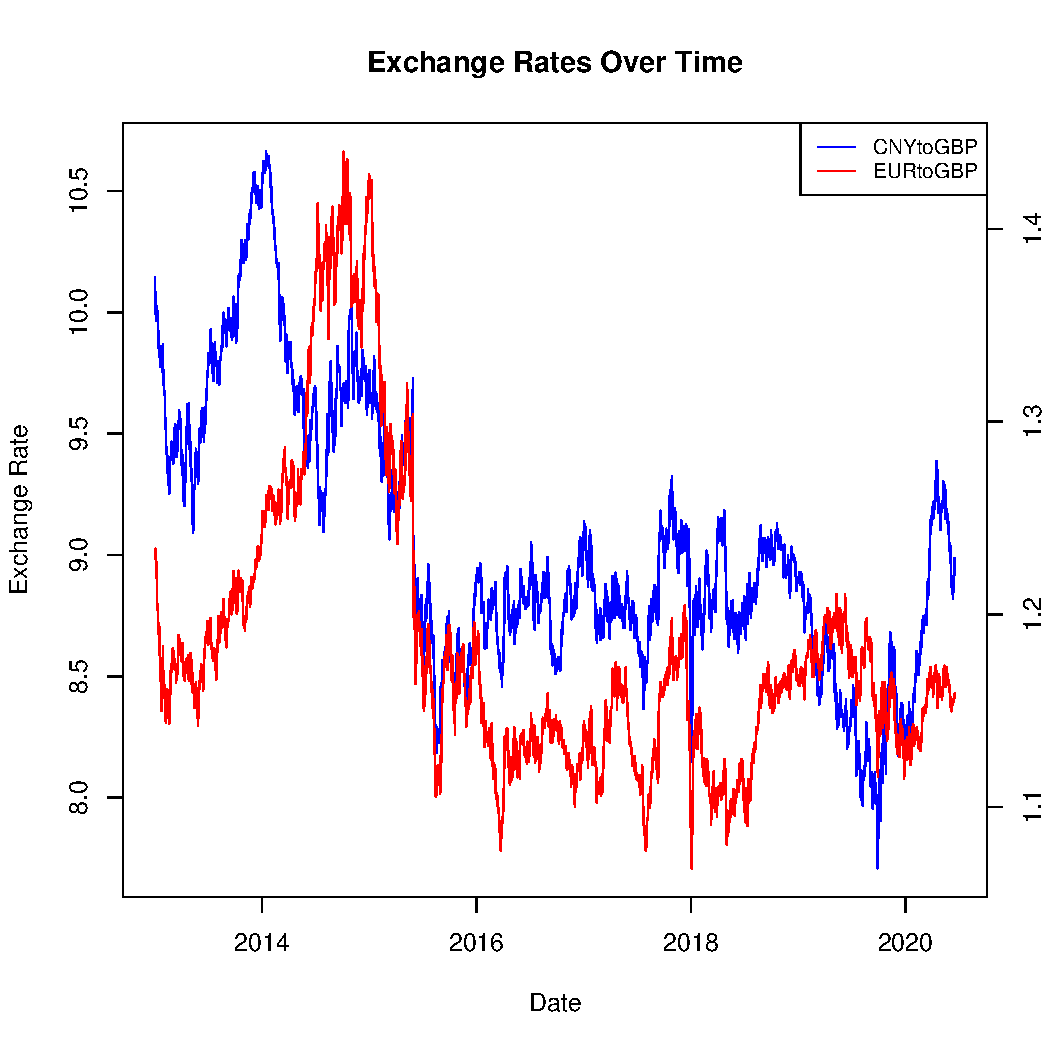
\includegraphics[width=\maxwidth]{figure/unnamed-chunk-4-1} \caption[Decomposition of addictive time series model]{Decomposition of addictive time series model}\label{fig:unnamed-chunk-4}
\end{figure}

\end{knitrout}

Hence, in this way, we will be able to view the seasonal trend and overall trend of CNY to GBP obviously.

\subsubsection{Double y-axis time series plot.}

If we want to display two different time series that measure two different quantities at the same time points, we can draw the second series again on the second Y-axis on the right side.

\begin{knitrout}
\definecolor{shadecolor}{rgb}{0.969, 0.969, 0.969}\color{fgcolor}\begin{kframe}
\begin{alltt}
\hlcom{# Plot of double y-axis time series}

\hlcom{# Plot the first time series with its y-axis}
\hlkwd{plot}\hlstd{(MyData}\hlopt{$}\hlstd{CNYtoGBP,} \hlkwc{type}\hlstd{=}\hlstr{"l"}\hlstd{,} \hlkwc{col}\hlstd{=}\hlstr{"blue"}\hlstd{,} \hlkwc{ylab}\hlstd{=}\hlstr{"Exchange Rate"}\hlstd{,} \hlkwc{xlab}\hlstd{=}\hlstr{"Date"}\hlstd{,}
     \hlkwc{main}\hlstd{=}\hlstr{"Exchange Rates Over Time"}\hlstd{)}

\hlcom{# Add the second time series with a secondary y-axis}
\hlkwd{par}\hlstd{(}\hlkwc{new}\hlstd{=}\hlnum{TRUE}\hlstd{)}
\hlkwd{plot}\hlstd{(ts_data}\hlopt{$}\hlstd{EURtoGBP,} \hlkwc{type}\hlstd{=}\hlstr{"l"}\hlstd{,} \hlkwc{col}\hlstd{=}\hlstr{"red"}\hlstd{,} \hlkwc{axes}\hlstd{=}\hlnum{FALSE}\hlstd{,} \hlkwc{xlab}\hlstd{=}\hlnum{NA}\hlstd{,} \hlkwc{ylab}\hlstd{=}\hlnum{NA}\hlstd{)}
\hlkwd{axis}\hlstd{(}\hlkwc{side}\hlstd{=}\hlnum{4}\hlstd{)}  \hlcom{# Add the secondary y-axis on the right}
\hlkwd{mtext}\hlstd{(}\hlstr{"Temp"}\hlstd{,} \hlkwc{side}\hlstd{=}\hlnum{4}\hlstd{,} \hlkwc{line}\hlstd{=}\hlnum{3}\hlstd{)}  \hlcom{# Label the secondary y-axis}

\hlcom{# Add a legend to distinguish the two time series}
\hlkwd{legend}\hlstd{(}\hlstr{"topright"}\hlstd{,} \hlkwc{legend}\hlstd{=}\hlkwd{c}\hlstd{(}\hlstr{"CNYtoGBP"}\hlstd{,} \hlstr{"EURtoGBP"}\hlstd{),}
       \hlkwc{col}\hlstd{=}\hlkwd{c}\hlstd{(}\hlstr{"blue"}\hlstd{,} \hlstr{"red"}\hlstd{),} \hlkwc{lty}\hlstd{=}\hlnum{1}\hlstd{,} \hlkwc{cex}\hlstd{=}\hlnum{0.8}\hlstd{)}
\end{alltt}
\end{kframe}\begin{figure}
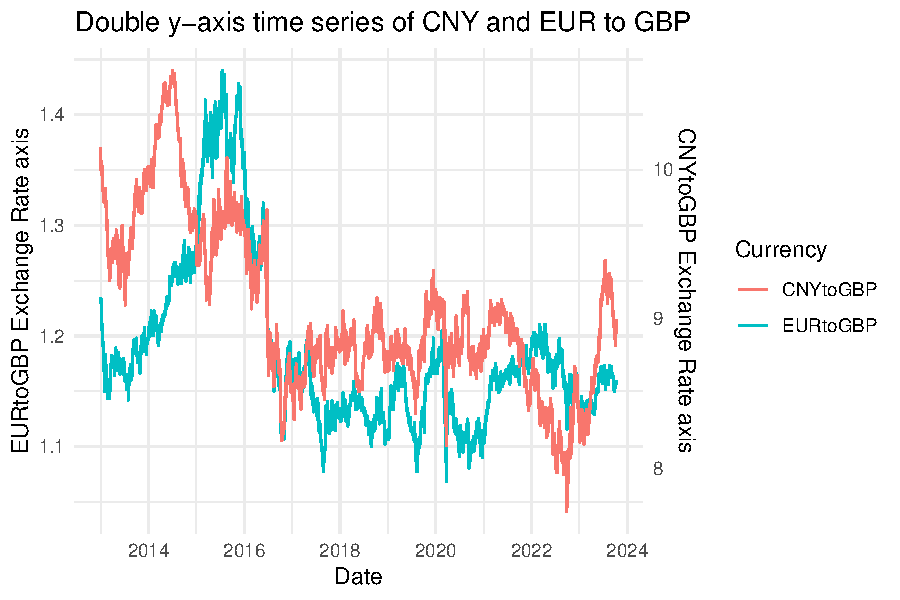
\includegraphics[width=\maxwidth]{figure/unnamed-chunk-5-1} \caption[Double y-axis time series]{Double y-axis time series}\label{fig:unnamed-chunk-5}
\end{figure}

\end{knitrout}

\subsubsection{Identification of anomalies}

A common approach to anomaly detection in time series data is to use the Z-score. The Z-score measures how many standard deviations a data point is from the mean. Data points with a Z-score above a certain threshold (e.g., 2 or 3) can be considered anomalies.

\begin{knitrout}
\definecolor{shadecolor}{rgb}{0.969, 0.969, 0.969}\color{fgcolor}\begin{kframe}
\begin{alltt}
\hlcom{#Plot of time series with anomalies}

\hlcom{# Calculate the Z-scores for the EURtoGBP exchange rate}
\hlstd{eur_to_gbp_series} \hlkwb{<-} \hlstd{MyData}\hlopt{$}\hlstd{EURtoGBP}
\hlstd{mean_val} \hlkwb{<-} \hlkwd{mean}\hlstd{(eur_to_gbp_series,} \hlkwc{na.rm} \hlstd{=} \hlnum{TRUE}\hlstd{)}
\hlstd{std_val} \hlkwb{<-} \hlkwd{sd}\hlstd{(eur_to_gbp_series,} \hlkwc{na.rm} \hlstd{=} \hlnum{TRUE}\hlstd{)}
\hlstd{z_scores} \hlkwb{<-} \hlkwd{abs}\hlstd{((eur_to_gbp_series} \hlopt{-} \hlstd{mean_val)} \hlopt{/} \hlstd{std_val)}

\hlcom{# Define a threshold for anomalies (e.g., Z-score > 2)}
\hlstd{threshold} \hlkwb{<-} \hlnum{3}
\hlstd{anomalies} \hlkwb{<-} \hlkwd{which}\hlstd{(z_scores} \hlopt{>} \hlstd{threshold)}

\hlstd{plot_data} \hlkwb{<-} \hlkwd{data.frame}\hlstd{(}\hlkwc{Date} \hlstd{=  MyData}\hlopt{$}\hlstd{Date,}
                        \hlkwc{Rate} \hlstd{= eur_to_gbp_series,}
                        \hlkwc{Anomaly} \hlstd{=} \hlkwd{ifelse}\hlstd{(z_scores} \hlopt{>} \hlstd{threshold,}
                                         \hlstd{eur_to_gbp_series,} \hlnum{NA}\hlstd{))}

\hlkwd{ggplot}\hlstd{(plot_data,} \hlkwd{aes}\hlstd{(}\hlkwc{x} \hlstd{= Date,} \hlkwc{y} \hlstd{= Rate))} \hlopt{+}
  \hlkwd{geom_line}\hlstd{(}\hlkwd{aes}\hlstd{(}\hlkwc{color} \hlstd{=} \hlstr{"EURtoGBP"}\hlstd{))} \hlopt{+}
  \hlkwd{geom_point}\hlstd{(}\hlkwd{aes}\hlstd{(}\hlkwc{y} \hlstd{= Anomaly,} \hlkwc{color} \hlstd{=} \hlstr{"Anomalies"}\hlstd{),} \hlkwc{na.rm} \hlstd{=} \hlnum{TRUE}\hlstd{)} \hlopt{+}
  \hlkwd{labs}\hlstd{(}\hlkwc{title} \hlstd{=} \hlstr{"EURtoGBP Exchange Rate with Anomalies Highlighted"}\hlstd{,}
       \hlkwc{y} \hlstd{=} \hlstr{"Exchange Rate to GBP"}\hlstd{,}
       \hlkwc{color} \hlstd{=} \hlstr{"Legend"}\hlstd{)} \hlopt{+}
  \hlkwd{scale_color_manual}\hlstd{(}\hlkwc{values} \hlstd{=} \hlkwd{c}\hlstd{(}\hlstr{"EURtoGBP"} \hlstd{=} \hlstr{"blue"}\hlstd{,}
                                \hlstr{"Anomalies"} \hlstd{=} \hlstr{"red"}\hlstd{))}
\end{alltt}
\end{kframe}\begin{figure}
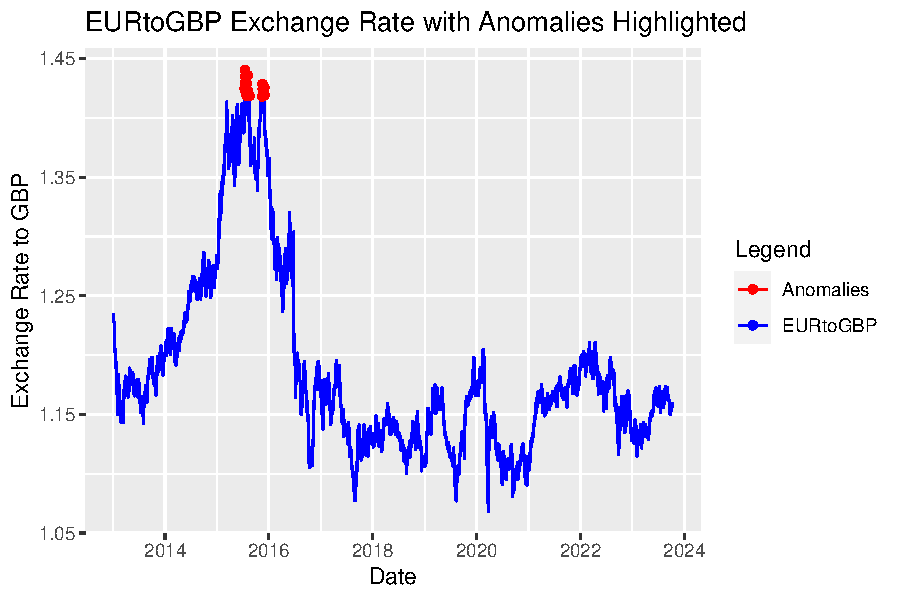
\includegraphics[width=\maxwidth]{figure/unnamed-chunk-6-1} \caption[Time series with anomalies]{Time series with anomalies}\label{fig:unnamed-chunk-6}
\end{figure}

\end{knitrout}


\subsection{Network Graphs}
\textbf{Definition and Utility:}
Network graphs, often referred to as graphs or networks, are a powerful data visualization method used to depict relationships between entities. These entities, known as nodes, are interconnected by edges or links, which represent relationships, connections, or interactions. Network graphs find extensive utility in various fields, such as social network analysis, transportation systems, and even biological networks like protein-protein interactions. They excel at revealing complex dependencies and structures, making them a critical tool for understanding relational data.

\subsubsection{The Mathematics behind Network Graphs:}
Constructing network graphs involves several mathematical intricacies. Here we present just a few of the many concepts that play a role in the creation of such graphs:
\begin{enumerate}
\item \textbf{Nodes and Edges}: Mathematically, a network graph, \(G\), is defined as \(G = (V, E)\), where \(V\) represents the set of nodes and \(E\) represents the set of edges connecting these nodes.
\item \textbf{Node Degree}: The degree of a node is the number of edges connected to it. In a directed graph, nodes can have both in-degrees and out-degrees.
\item \textbf{Centrality Measures}: Centrality metrics like degree centrality, betweenness centrality, and closeness centrality provide insights into the relative importance or influence of nodes within a network.
\item \textbf{Graph Metrics}: Graph theory concepts like shortest paths, connected components, and clustering coefficients are used to analyze the network's structure.
\end{enumerate}

\textbf{Formulas used in Network Graphs:}

\begin{enumerate}
\item \textbf{Degree of a Node (Undirected Graph)}:
\[
\text{Degree}(v) = \sum_{w \in V} A(v, w)
\]
where \(A(v, w)\) is the adjacency matrix element, indicating whether there is a connection between nodes \(v\) and \(w\).
\item \textbf{Degree of a Node (Directed Graph)}:
\[
\text{In-Degree}(v) = \sum_{w \in V} A(w, v)
\]
\[
\text{Out-Degree}(v) = \sum_{w \in V} A(v, w)
\]
\item \textbf{Betweenness Centrality (for unweighted graphs)}:
\[
C_B(v) = \sum_{s \neq v \neq t} \frac{\sigma_{st}(v)}{\sigma_{st}}
\]
where \(\sigma_{st}\) is the number of shortest paths from node \(s\) to \(t\), and \(\sigma_{st}(v)\) is the number of those paths passing through node \(v\).
\end{enumerate}

\subsubsection{Network Graphs in Practice}




\begin{figure}[h]
\centering
\begin{knitrout}
\definecolor{shadecolor}{rgb}{0.969, 0.969, 0.969}\color{fgcolor}\begin{kframe}
\begin{alltt}
\hlcom{# Plot the graph}
\hlcom{#plot(lesmis_graph, layout = layout, vertex.label.cex = 0.7, main = "Character Interactions in Les Misérables")}
\end{alltt}
\end{kframe}
\end{knitrout}
\end{figure}

\subsection{Sankey Diagrams}
xxx

\subsection{Geographic Maps and Spatial Data Visualisation}

\text{https://data.london.gov.uk/dataset/statistical-gis-boundary-files-london#:~:text=,2014.zip%20%283.84%20MB%29%20From}\\
\text{https://data.london.gov.uk/dataset/recorded_crime_summary#:~:text=Recorded%20Crime%3A%20Geographic%20Breakdown,covering%20all%20historic%20full}\\
\text{https://public.tableau.com/app/profile/metropolitan.police.service/viz/MonthlyCrimeDataNewCats/Coversheet}\\
\text{https://medium.com/@davemorison/an-interactive-visualization-of-londons-crime-data-using-shiny-applications-and-r-7ca9011e064b?source=author_recirc-----8dcefef1c397----0---------------------07ef707d_5478_4230_b6e6_451582a6cc55-------}

\begin{knitrout}
\definecolor{shadecolor}{rgb}{0.969, 0.969, 0.969}\color{fgcolor}\begin{kframe}
\begin{alltt}
\hlcom{# Load the shapefile}
\hlstd{london_boroughs} \hlkwb{<-} \hlkwd{st_read}\hlstd{(}\hlstr{"London_Ward.shp"}\hlstd{)}
\end{alltt}
\begin{verbatim}
## Reading layer `London_Ward' from data source 
##   `C:\Users\chuyu\Downloads\Data-Visualisation-Project\London_Ward.shp' 
##   using driver `ESRI Shapefile'
## Simple feature collection with 657 features and 6 fields
## Geometry type: POLYGON
## Dimension:     XY
## Bounding box:  xmin: 503568.2 ymin: 155850.8 xmax: 561957.5 ymax: 200933.9
## Projected CRS: OSGB36 / British National Grid
\end{verbatim}
\begin{alltt}
\hlcom{# Load the crime data (assuming it's in CSV format)}
\hlstd{crime_data} \hlkwb{<-} \hlkwd{read.csv}\hlstd{(}\hlstr{"BoroughLevelCrime.csv"}\hlstd{)}

\hlcom{# Summing the total crimes for each borough over the entire timeframe}
\hlstd{borough_totals} \hlkwb{<-} \hlstd{crime_data} \hlopt
  \hlkwd{group_by}\hlstd{(LookUp_BoroughName)} \hlopt
  \hlkwd{summarise}\hlstd{(}\hlkwc{Total_Crimes} \hlstd{=} \hlkwd{sum}\hlstd{(}\hlkwd{across}\hlstd{(}\hlkwd{starts_with}\hlstd{(}\hlstr{"X2020"}\hlstd{))))}

\hlcom{# Merge the crime data with the shapefile}
\hlstd{merged_data} \hlkwb{<-} \hlkwd{merge}\hlstd{(london_boroughs, borough_totals,}
                     \hlkwc{by.x}\hlstd{=}\hlstr{"DISTRICT"}\hlstd{,} \hlkwc{by.y}\hlstd{=}\hlstr{"LookUp_BoroughName"}\hlstd{)}

\hlcom{# Aggregate geometries by district}
\hlstd{aggregated_data} \hlkwb{<-} \hlstd{merged_data} \hlopt
  \hlkwd{group_by}\hlstd{(DISTRICT)} \hlopt
  \hlkwd{summarise}\hlstd{(}\hlkwc{geometry} \hlstd{=} \hlkwd{st_union}\hlstd{(geometry),} \hlkwc{Total_Crimes} \hlstd{=} \hlkwd{first}\hlstd{(Total_Crimes))}

\hlcom{# Calculate centroids for labeling}
\hlstd{aggregated_data}\hlopt{$}\hlstd{centroid} \hlkwb{<-} \hlkwd{st_centroid}\hlstd{(aggregated_data}\hlopt{$}\hlstd{geometry)}
\end{alltt}
\end{kframe}
\end{knitrout}


\begin{knitrout}
\definecolor{shadecolor}{rgb}{0.969, 0.969, 0.969}\color{fgcolor}\begin{kframe}
\begin{alltt}
\hlcom{# Plot the Crime numbers in London by boroughs}
\hlstd{plot} \hlkwb{<-} \hlkwd{ggplot}\hlstd{(}\hlkwc{data}\hlstd{=aggregated_data)} \hlopt{+}
  \hlkwd{geom_sf}\hlstd{(}\hlkwd{aes}\hlstd{(}\hlkwc{fill}\hlstd{=Total_Crimes))} \hlopt{+}
  \hlkwd{geom_sf_text}\hlstd{(}\hlkwd{aes}\hlstd{(}\hlkwc{label} \hlstd{= DISTRICT,} \hlkwc{geometry} \hlstd{= centroid),}
               \hlkwc{size} \hlstd{=} \hlnum{3}\hlstd{,} \hlkwc{check_overlap} \hlstd{=} \hlnum{TRUE}\hlstd{)} \hlopt{+}
  \hlkwd{scale_fill_gradient}\hlstd{(}\hlkwc{low}\hlstd{=}\hlstr{"Green"}\hlstd{,} \hlkwc{high}\hlstd{=}\hlstr{"red"}\hlstd{)} \hlopt{+}
  \hlkwd{theme_minimal}\hlstd{()} \hlopt{+}
  \hlkwd{labs}\hlstd{(}\hlkwc{title}\hlstd{=}\hlstr{"Total Crime by Borough in London (April 2010 - September 2021)"}\hlstd{,}
       \hlkwc{fill}\hlstd{=}\hlstr{"Total Crimes"}\hlstd{)}

\hlkwd{print}\hlstd{(plot)}
\end{alltt}
\end{kframe}
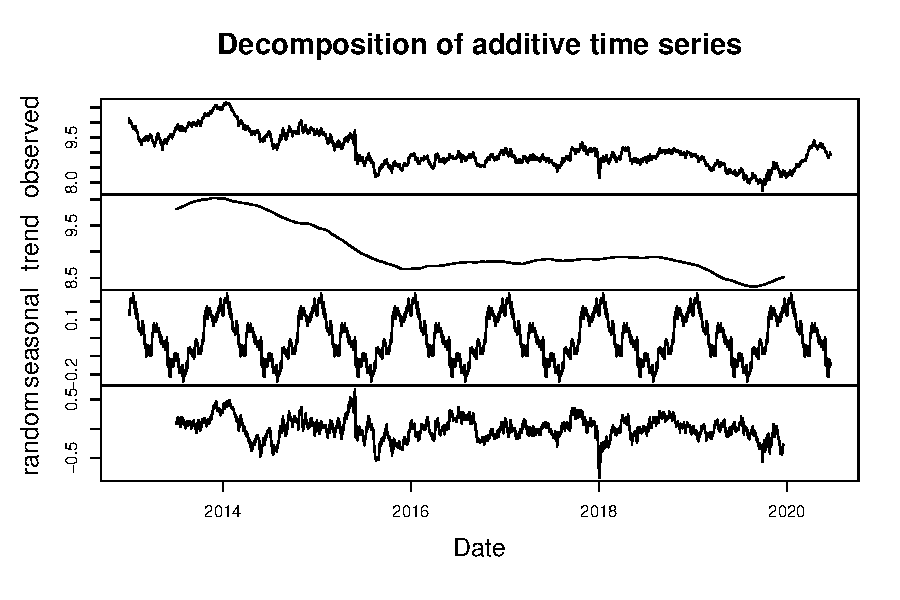
\includegraphics[width=\maxwidth]{figure/unnamed-chunk-8-1} 
\end{knitrout}

\subsection{3D and Interactive Visualisations}
ggplot2 is one of the most popular data visualization libraries in R, but it is primarily designed for 2D data visualization. Directly creating 3D views with ggplot2 can be challenging.

rgl: This is a widely-used package for 3D visualizations. It allows you to create interactive 3D scatter plots, line plots, and more, and view them in a separate window.

3D data visualization is an approach that employs three-dimensional graphics to represent complex data structures, allowing for an immersive exploration of information. Unlike traditional 2D visualizations (like bar graphs or line charts), 3D visualizations can convey an additional dimension of data, making them particularly valuable in specific contexts.

Our first example will be  a scatter plot. We can use scatterplot3d package  to help us for data visualization.
\section{Trees Dataset in R}

The \texttt{trees} dataset is one of R's built-in datasets. It contains measurements from 31 felled black cherry trees and provides insights into the relationship between a tree's girth, its height, and the volume of timber it can produce. The dataset comprises the following variables:

\begin{itemize}
    \item \textbf{Girth:} The diameter of the tree, measured in inches at 4 ft 6 in above the ground.
    \item \textbf{Height:} The height of the tree, measured in feet.
    \item \textbf{Volume:} The volume of timber, measured in cubic feet, that the tree can produce.
\end{itemize}
\begin{knitrout}
\definecolor{shadecolor}{rgb}{0.969, 0.969, 0.969}\color{fgcolor}\begin{kframe}
\begin{alltt}
\hlkwd{data}\hlstd{(trees)}
\hlcom{# Generate colors based on the Volume variable}
\hlstd{colors} \hlkwb{<-} \hlkwd{colorRampPalette}\hlstd{(}\hlkwd{c}\hlstd{(}\hlstr{"blue"}\hlstd{,} \hlstr{"red"}\hlstd{))(}\hlkwd{length}\hlstd{(}\hlkwd{unique}\hlstd{(trees}\hlopt{$}\hlstd{Volume)))}
\hlstd{color_assign} \hlkwb{<-} \hlstd{colors[}\hlkwd{as.numeric}\hlstd{(}\hlkwd{as.factor}\hlstd{(trees}\hlopt{$}\hlstd{Volume))]}
\hlcom{# Create 3d scatter plot with colors}
\hlkwd{scatterplot3d}\hlstd{(trees}\hlopt{$}\hlstd{Girth, trees}\hlopt{$}\hlstd{Height, trees}\hlopt{$}\hlstd{Volume,}
              \hlkwc{color}\hlstd{=color_assign,}
              \hlkwc{main}\hlstd{=}\hlstr{"3D Scatterplot of trees data"}\hlstd{,}
              \hlkwc{xlab}\hlstd{=}\hlstr{"Girth (inches)"}\hlstd{,}
              \hlkwc{ylab}\hlstd{=}\hlstr{"Height (ft)"}\hlstd{,}
              \hlkwc{zlab}\hlstd{=}\hlstr{"Volume (cubic ft)"}\hlstd{)}
\end{alltt}
\end{kframe}\begin{figure}
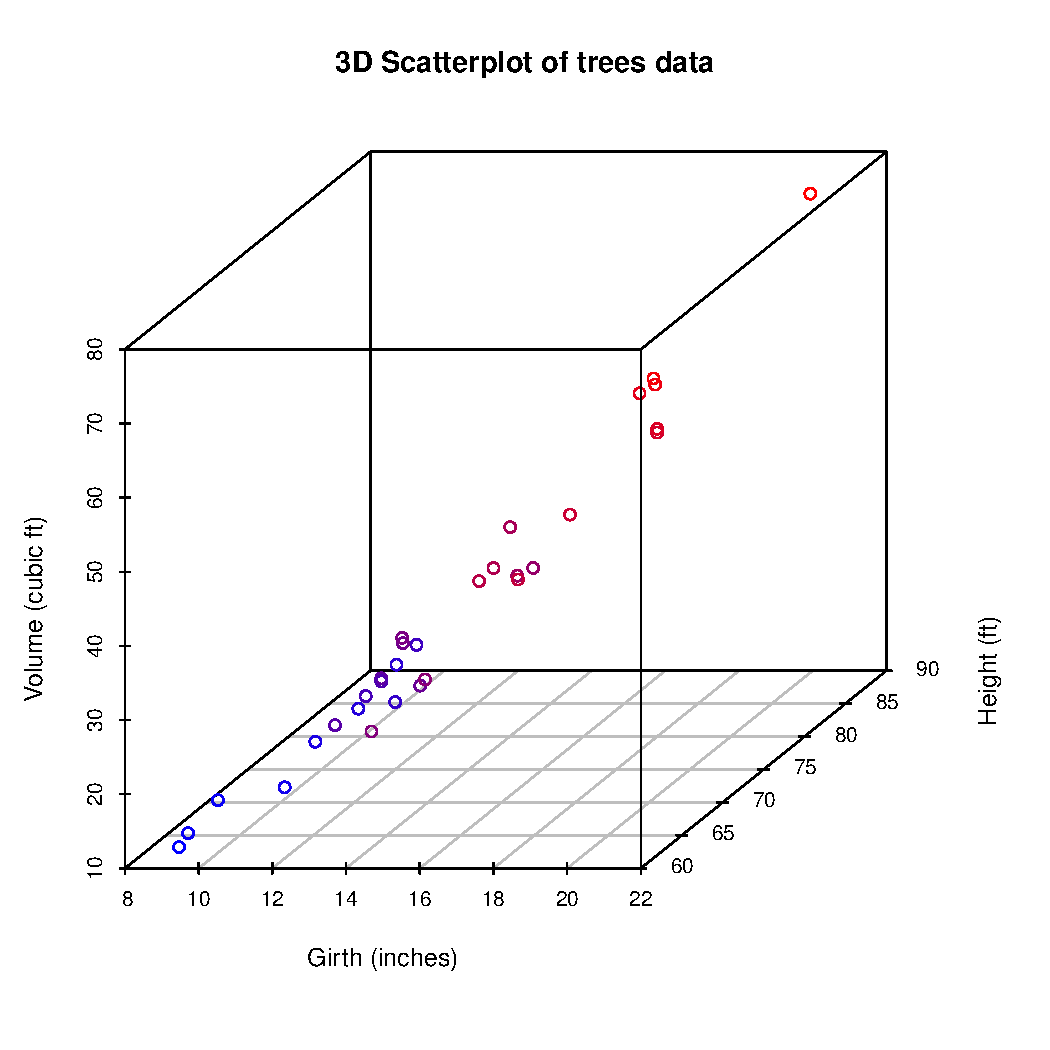
\includegraphics[width=\maxwidth]{figure/3d1-1} \caption[3d scatter plot]{3d scatter plot}\label{fig:3d1}
\end{figure}

\end{knitrout}




\subsection{Advanced Visualisation Techniques}
xxx




\section{Practical Implementations}
XXX




\section{Case Studies}
\subsection{Market Analysis Dashboards}
XXX
\subsection{Healthcare Data Visualisation}
XXX




\section{State-of-the-Art Approaches}
XXX


\section{Conclusion}

XXX

\end{document}
